\documentclass[conference]{IEEEtran}
\usepackage[T1]{fontenc}
\usepackage[utf8]{inputenc}
\usepackage[spanish,es-nodecimaldot]{babel}
\usepackage{graphicx,booktabs,amsmath,amssymb,array,url}
\graphicspath{{results/}}
\title{Evaluación externa de explicaciones de redes convolucionales mediante perturbaciones pulmonares en radiografías con hallazgos compatibles con tuberculosis}
\author{\IEEEauthorblockN{Alexandra Cristal Salazar Gisberth}
\IEEEauthorblockA{Carrera de Informática, Facultad de Ciencias Puras y Naturales\\Universidad Mayor de San Andrés, La Paz, Bolivia}}
\begin{document}
\maketitle
\begin{abstract}
Se evaluó retrospectivamente si la puntuación positiva de dos clasificadores de radiografías dependía más de una región con hallazgos anotados que de regiones sin anotación del mismo pulmón. Se utilizaron DenseNet121 y ResNet50 entrenadas en Shenzhen con tres semillas y evaluadas en Montgomery. De 55 radiografías positivas anotadas, 17 permitieron trasladar la forma digital de una caja índice a por lo menos tres controles del mismo pulmón y tercio vertical. Se comparó la caída del logit positivo menos el normal tras un desenfoque idéntico en cada región. En DenseNet121, la mediana de la diferencia índice menos controles, promediada por radiografía entre semillas, fue 0,172 (IC bootstrap del 95\%: 0,065 a 0,632; Wilcoxon bilateral $p=0,010986$). En ResNet50 fue 0,064 (IC: $-0,005$ a 0,336). El resultado principal es exploratorio, está condicionado a la elegibilidad geométrica y no establece causalidad clínica ni validez diagnóstica de un dispositivo.
\end{abstract}
\begin{IEEEkeywords}
tuberculosis, radiografía de tórax, explicabilidad, Grad-CAM, perturbación, evaluación externa
\end{IEEEkeywords}
\begin{abstract}
\textbf{Abstract---} A retrospective analysis examined whether the positive-class score of two chest radiograph classifiers depended more on an annotated finding region than on unannotated regions in the same lung. DenseNet121 and ResNet50 were trained on Shenzhen with three seeds and evaluated on Montgomery. Of 55 annotated positive radiographs, 17 allowed an index-box digital shape to be translated to at least three same-lung, same-vertical-third controls. The difference in positive-minus-normal logit drop after identical blurring was computed per image. For DenseNet121, the median index-minus-control difference averaged across seeds was 0.172 (95\% bootstrap CI: 0.065 to 0.632; two-sided Wilcoxon $p=0.010986$). For ResNet50 it was 0.064 (CI: $-0.005$ to 0.336). This exploratory result is restricted by geometric eligibility and does not establish clinical causality or device validity.
\end{abstract}

\section{Introducción}
En 2025, la Organización Mundial de la Salud estimó que 10,6 millones de personas desarrollaron tuberculosis y que 1,13 millones fallecieron por esta enfermedad en el mundo \cite{who2026}. La OMS considera la lectura de radiografías mediante detección asistida por computadora una vía de cribado para identificar personas que podrían beneficiarse de pruebas adicionales \cite{whocad2025}. Un clasificador experimental de imágenes retrospectivas, sin estándar microbiológico ni evaluación prospectiva, no equivale a uno de los productos examinados en esa política.

Las colecciones públicas Shenzhen y Montgomery etiquetan radiografías normales y anormales con manifestaciones \emph{compatibles} con tuberculosis (TB) \cite{jaeger2014,nlmdata}. Esa etiqueta no acredita tuberculosis activa confirmada. La distinción importa al interpretar explicaciones: que un mapa coincida con una caja radiológica no demuestra que el modelo haya reconocido una entidad histopatológica; que la salida cambie al alterar píxeles tampoco demuestra qué ocurriría ante una intervención clínica. Se observó anteriormente una caída de discriminación entre Shenzhen y Montgomery y concentración parcial de mapas dentro de los pulmones. Se formuló entonces una pregunta operacional adicional: ¿cuánto cambia la puntuación positiva al perturbar una región anotada, frente a regiones de control comparables de la \emph{misma} radiografía y pulmón?

El objetivo de esta extensión retrospectiva con evaluación externa fue estimar esa diferencia pareada y relacionarla, de forma secundaria, con la masa de Grad-CAM. Montgomery había sido estudiado en el borrador previo; por ello el contraste es exploratorio en una cohorte externa ya conocida. Una replicación requerirá imágenes independientes y compatibles.

\section{Marco teórico}
\subsection{Representación convolucional y transferencia}
Una red convolucional aplica filtros locales que comparten parámetros. La composición de capas amplía el campo receptivo efectivo, mientras que la reducción espacial disminuye el detalle de localización. El aprendizaje por transferencia parte de filtros ajustados en ImageNet, pero no asegura que sus representaciones sean adecuadas para radiografías. DenseNet concatena características de capas anteriores, facilitando su reutilización \cite{huang2017}; ResNet incorpora sumas residuales que facilitan la optimización de redes profundas \cite{he2016}. Se fijó DenseNet121 como arquitectura principal por continuidad con el estudio original y ResNet50 como sensibilidad arquitectónica.

La operación convolucional construye respuestas a patrones locales; capas profundas combinan bordes, texturas y formas en patrones de escala mayor. La reducción por paso o agrupación incrementa la invariancia aproximada a pequeños desplazamientos, pero pierde información de posición. Una decisión de imagen completa puede depender de una estructura extensa aunque su mapa de activación final sea grueso. Al interpolar ese mapa a la resolución original se recupera una cuadrícula visualmente continua, no el detalle espacial perdido. Esta distinción es especialmente relevante para cajas pequeñas de hallazgos: un mapa amplio puede concentrar masa en una región pulmonar y fallar al señalar el máximo dentro de la caja.

El preentrenamiento en ImageNet inicializa filtros y conexiones, y la adaptación con imágenes de Shenzhen modifica esos parámetros mediante la pérdida de clasificación. La concatenación en DenseNet permite que características tempranas y tardías coexistan explícitamente en capas posteriores. La suma residual en ResNet aprende una corrección sobre una ruta de identidad; el mecanismo de conexión y la distribución de representaciones resultantes difieren de DenseNet. Por ello, una diferencia entre ambas redes en Montgomery puede reflejar arquitectura, optimización o semilla, y no se atribuye a un único mecanismo sin un experimento diseñado para aislarlo.

\subsection{Grad-CAM y LIME como explicaciones locales}
Grad-CAM combina mapas de activación de una capa convolucional mediante pesos obtenidos de gradientes de una clase objetivo \cite{selvaraju2017}. Su resolución depende de la capa elegida y puede perder focos pequeños. LIME aproxima localmente la salida mediante superpíxeles perturbados y una regresión ponderada \cite{ribeiro2016}; depende de la segmentación, el muestreo y el fondo elegido. Un mapa nulo no contiene un máximo interpretable y se registra por separado. En el análisis general histórico se explicó la clase \emph{predicha}; en el análisis histórico de cajas y en esta extensión se fijó la clase \emph{positiva}, incluidos los falsos negativos. Los resultados de ambas definiciones no son intercambiables.

Si $A^k$ es el mapa de activación del canal $k$ y $z_c$ la salida de la clase $c$, Grad-CAM utiliza pesos proporcionales a la media espacial de $\partial z_c/\partial A^k$. La suma ponderada de canales se rectifica y se interpola sobre la imagen. El mapa resultante indica qué posiciones de esa capa contribuyen al logit objetivo bajo la linealización local de la red; no es una segmentación supervisada de la enfermedad. Una zona de alta relevancia puede ser normal, y una caja anotada puede contener información que no resulte decisiva para el clasificador.

LIME divide la imagen en superpíxeles y evalúa variaciones en las que algunos se sustituyen por un fondo. Ajusta un modelo simple alrededor del caso, ponderando más las perturbaciones próximas a la imagen original. Los coeficientes positivos del sustituto indican asociaciones locales con la clase objetivo; la fidelidad del sustituto y el aspecto de los superpíxeles dependen de las perturbaciones elegidas. Una comparación visual entre LIME y Grad-CAM requiere fijar la misma clase, radiografía y peso del clasificador. Incluso entonces, las regiones coloreadas no son probabilidades de lesión y los dos métodos resumen mecanismos matemáticos diferentes.

\subsection{Discriminación, localización y fidelidad}
La discriminación (ROC-AUC y precisión promedio), una decisión con umbral fijo y la calibración son propiedades distintas. La puntuación de Brier resume error probabilístico, pero por sí sola tampoco caracteriza toda la calibración. Para XAI se separaron localización anatómica, fidelidad por perturbación, sensibilidad a pesos y estabilidad entre semillas. Una caída de AUC al cambiar de colección es compatible con cambio de dominio; no identifica por sí sola un atajo aprendido. Este riesgo ha sido documentado en radiografía torácica y en detectores de COVID-19 \cite{zech2018,degrave2021}.

ROC-AUC mide la probabilidad de que una radiografía positiva reciba una puntuación mayor que una negativa elegidas al azar; no fija un umbral operativo. La precisión promedio (AP) suma la precisión al aumentar el recobrado y depende de la prevalencia de la clase positiva. Sensibilidad y especificidad cuantifican errores distintos en un umbral dado; F1 combina precisión y recobrado, mientras que MCC incorpora las cuatro celdas de la matriz de confusión y resulta informativo ante desbalance. Brier promedia $(p_i-y_i)^2$ para evaluar el error cuadrático de probabilidades. Un AUC similar en dos modelos puede coexistir con sensibilidades o errores de probabilidad muy diferentes cuando se traslada un umbral desde otro dominio.

La energía intrapulmonar (EIL) es la fracción de intensidad no negativa del mapa dentro de la máscara pulmonar. La ganancia normalizada divide esa fracción por el área relativa del pulmón; vale uno para un mapa uniforme. La ganancia en una caja condicionada al pulmón aplica el mismo principio a la intersección entre caja y máscara. La tasa de acierto del máximo del mapa comprueba una sola posición, y el IoU entre el 10\% pulmonar más relevante y la región de referencia compara dos conjuntos de píxeles. Estas medidas no son equivalentes: la energía puede estar distribuida alrededor de la caja sin que su máximo caiga en ella. La cobertura de mapas válidos debe acompañar a cualquier promedio, porque excluir mapas nulos sin informarlo sesga la descripción.

Las curvas de eliminación sustituyen primero las posiciones más relevantes por un fondo definido; las de inserción restauran esas posiciones sobre un fondo alterado. Si la salida cambia mucho, se documenta dependencia de los píxeles bajo ese operador, pero no se identifica una causa clínica. La aleatorización de pesos examina si un mapa cambia con los parámetros aprendidos. La estabilidad entre semillas pregunta si la explicación depende de una realización del entrenamiento. Estas verificaciones se complementan: coincidencia anatómica, dependencia de salida, sensibilidad a pesos y estabilidad no se infieren una de otra.

\section{Trabajos relacionados}
Lakhani y Sundaram abordaron clasificación de TB en radiografías \cite{lakhani2017}; Rajaraman y colaboradores estudiaron anotaciones débiles de hallazgos y segmentación \cite{rajaraman2021}. La revisión de localización débil de TB recoge técnicas de oclusión y mapas \cite{weakreview2023}. Saporta y colaboradores compararon métodos de saliencia con referencia humana en radiografías \cite{saporta2022}, y Adebayo y colaboradores propusieron pruebas de sensibilidad a pesos para mapas \cite{adebayo2018}. La Tabla~\ref{tab:antecedentes} explicita qué control y unidad se utilizaron o, cuando el alcance del trabajo citado no permite afirmarlo, qué dimensión queda sin comparación directa. La búsqueda se realizó el 26 de noviembre de 2026 en NLM, PubMed, IEEE/CVF, Nature y buscadores académicos con ``tuberculosis chest radiograph matched lesion occlusion intrapulmonary control'', ``tuberculosis weak localization occlusion sensitivity'' y variantes. Se encontraron antecedentes de oclusión, pero no se verificó exhaustivamente una prioridad para el diseño pareado de lesión y regiones trasladadas del mismo pulmón. La contribución se presenta como extensión operacional del contraste previo pulmón--borde, sin reivindicación de primacía.

\begin{table*}[t]
\caption{Antecedentes y dimensión comparable al contraste propuesto. ``No determinado'' indica que la presente revisión no verificó esa propiedad; no implica ausencia en el estudio original.}
\label{tab:antecedentes}\centering\footnotesize
\begin{tabular}{p{2.3cm}p{3.0cm}p{3.1cm}p{3.0cm}p{2.5cm}}
\toprule
Trabajo & Tarea y conjunto & Referencia espacial & Perturbación o control & Unidad de análisis comunicada aquí\\\midrule
Lakhani y Sundaram \cite{lakhani2017} & Clasificación de TB en CXR & Etiqueta de imagen & Sin contraste intrapulmonar verificado & Radiografía\\
Rajaraman et al. \cite{rajaraman2021} & Segmentación de hallazgos compatibles con TB & Localizaciones débiles NLM & Sin pares trasladados verificados & Imagen/anotación\\
Revisión TB \cite{weakreview2023} & Localización débil en CXR & Variable entre estudios & Incluye oclusión; diseños heterogéneos & Variable\\
Saporta et al. \cite{saporta2022} & Saliencia en CXR multietiqueta & Segmentación humana & Comparación de métodos & Radiografía\\
Adebayo et al. \cite{adebayo2018} & Validez de mapas & Dependencia de parámetros & Pesos aleatorizados & Mapa/modelo\\
DeGrave et al. \cite{degrave2021} & COVID-19 en CXR & Interpretación de atajos & Comparación de señal y atajos & Radiografía/cohorte\\
\bottomrule
\end{tabular}
\end{table*}

\section{Datos y método}
\subsection{Procedencia, partición y modelos}
Las radiografías se recuperaron de la copia local de la versión 1 de \emph{Pulmonary Chest X-Ray Abnormalities} en Kaggle \cite{kaggle}; la fuente de las colecciones y las anotaciones auxiliares fue la NLM \cite{nlmdata}. La auditoría local registró 662 imágenes de Shenzhen (326 normales, 336 anormales) y 138 de Montgomery (80 normales, 58 anormales), con pares de máscaras izquierda y derecha para las 138. Se verificaron identificadores de radiografía únicos y la correspondencia de máscaras. El conjunto de entrenamiento, validación y prueba interna de Shenzhen fue de 462, 67 y 133 imágenes con estratificación y semilla 42; el manifiesto histórico se conservó. No se dispuso de un identificador independiente de paciente que permitiera demostrar agrupación por paciente. Montgomery se reservó para prueba externa, sin seleccionar pesos, hiperparámetros o umbral. Las cajas de consenso NLM abarcaron 109 anotaciones en 55 radiografías positivas de Montgomery, definidas sobre la referencia de 1024$\times$1024 píxeles \cite{nlmdata,rajaraman2021}; se escalaron a 224$\times$224 mediante piso para los límites iniciales y techo para los finales. Las máscaras binarias se redimensionaron con vecino más cercano. Las cajas son aproximaciones, no contornos de enfermedad.

Se reutilizaron los seis pesos ya entrenados en el estudio original: DenseNet121 y ResNet50 con semillas 0, 1 y 2, inicialización de ImageNet, ajuste completo con AdamW ($10^{-4}$), lote de 4 y acumulación de 8, hasta 20 épocas, parada temprana con paciencia 5 y AUC de validación. Las imágenes en grises se replicaron a tres canales, se redimensionaron a 224$\times$224 y se normalizaron con estadísticas de ImageNet. Los umbrales se seleccionaron mediante Youden exclusivamente en validación de Shenzhen y permanecieron fijos en ambas pruebas. La inferencia de la ampliación se realizó con pesos congelados.

\subsection{Selección geométrica previa a la inferencia}
Por cada radiografía positiva anotada se eligió la caja cuya intersección con un solo pulmón tuviera más píxeles. El desempate fue pulmón izquierdo, luego orden del CSV. La región índice debía cubrir al menos 50\% de la caja y contener 25 píxeles. La máscara de la intersección se trasladó sin cambiar forma ni número de píxeles a posiciones completamente incluidas en el mismo pulmón, en el mismo tercio vertical según el centroide y sin solapar ninguna caja anotada. La distancia media de los píxeles al borde pulmonar pudo diferir como máximo cinco píxeles de la región índice. Se ordenaron candidatos por esa diferencia, distancia vertical y horizontal al centroide, y coordenadas. Se conservaron hasta cinco controles con centroides separados al menos doce píxeles; se exigieron tres. Las reglas se ejecutaron sobre geometría antes de cargar salidas de los modelos. Las regiones de control se denominan \emph{sin anotación}: pueden contener hallazgos no marcados. El manifiesto de elegibilidad registra los descartes y distancias residuales.

De 55 imágenes anotadas, 17 cumplieron las reglas. Una no alcanzó el mínimo de cobertura/área; 37 no permitieron tres traslaciones elegibles. Esta fuerte selección limita la generalización del contraste a lesiones pequeñas y ubicaciones con espacio de control. La Fig.~\ref{fig:example} muestra una radiografía y la geometría usada; no se eligió a partir de la respuesta del modelo.

\begin{figure}[t]\centering
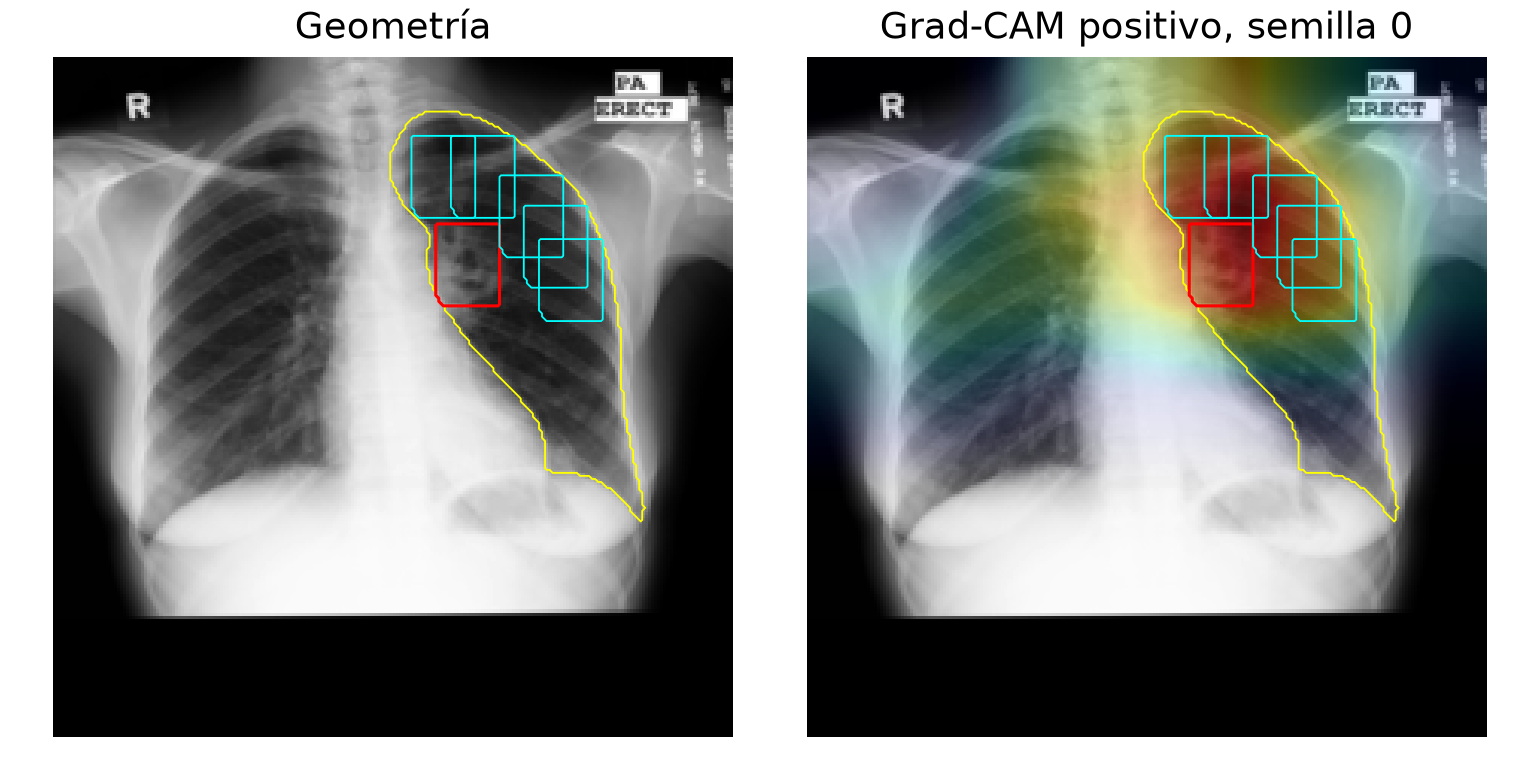
\includegraphics[width=\columnwidth]{fig_matched_example.png}
\caption{Primer caso elegible por identificador: pulmón (amarillo), región índice (rojo), controles (cian) y Grad-CAM positivo de DenseNet121 semilla 0. Los controles evitan las cajas anotadas.}\label{fig:example}
\end{figure}

\subsection{Perturbación y contraste}
Se generó una imagen completa desenfocada con filtro gaussiano de $\sigma=10$ píxeles y se sustituyeron solo los píxeles de cada máscara en una copia de la imagen original. La intensidad alternativa prefijada fue $\sigma=5$. Cada máscara fue exactamente del mismo tamaño en píxeles y se usó la misma normalización. Se verificó que una máscara vacía dejara la imagen intacta. Para cada modelo y semilla se definió
\begin{equation}
\begin{aligned}
s(x)&=z_1(x)-z_0(x),\\
\Delta(R)&=s(x)-s(x_R),\\
D&=\Delta(R_{\mathrm{ind}})-\operatorname{mediana}_j\Delta(R_j).
\end{aligned}
\end{equation}
Se promediaron los tres valores $D$ dentro de cada radiografía antes de la inferencia. $D>0$ indica que la puntuación de la clase positiva cayó más al intervenir la región índice que sus controles bajo este operador. El cambio de probabilidad fue secundario. La región índice se usó incluso cuando el modelo clasificó la imagen como negativa.

Para relacionar el contraste con XAI se calculó Grad-CAM de la clase positiva en las mismas imágenes y semillas, y la masa de mapa en la región índice menos la mediana de masa en los controles, condicionada a la suma pulmonar. Se registraron mapas nulos o sin masa pulmonar como inválidos. La concordancia entre esta diferencia de masa y $D$ se examinó mediante Spearman por radiografía, con IC bootstrap. Como diagnósticos descriptivos adicionales se calcularon mapas uniformes, diez mapas aleatorios suavizados por imagen con rejilla 7$\times$7 y un mapa gaussiano centrado fijo de ancho $0,2\times224$ píxeles. No se incluyeron en la prueba principal. También se calculó IoU entre el 10\% más relevante dentro del pulmón y la región índice, resolviendo empates por índice lineal del píxel.

Se obtuvieron curvas secundarias de eliminación e inserción de píxeles pulmonares ordenados por Grad-CAM, para fracciones $0,0$ a $0,5$ en pasos de $0,1$. Ambas usaron el mismo fondo pulmonar desenfocado con $\sigma=10$; fuera del pulmón se mantuvo la imagen original y la clase objetivo fue siempre la positiva. La eliminación partió de la imagen original y sustituyó los píxeles más relevantes por el fondo; la inserción partió del pulmón desenfocado y restauró esos píxeles originales. Las áreas bajo curvas se normalizaron por el intervalo de fracciones. Una menor área de eliminación y una mayor área de inserción sugieren mayor sensibilidad de la puntuación a las posiciones ordenadas, pero los extremos iniciales son distintos y las imágenes pueden estar fuera de distribución. El análisis histórico anterior aportó LIME en 40 casos de semilla 0 y aleatorización global de pesos en 55 casos; esas comparaciones tienen distinta cobertura y se identifican como tales.

Para facilitar la inspección visual se produjeron nuevas láminas con las cuatro primeras radiografías elegibles por identificador, sin seleccionar ejemplos según la forma del mapa. Se usó la semilla de entrenamiento 0 en cada arquitectura, Grad-CAM y LIME sobre la misma clase positiva, con 800 perturbaciones LIME, 60 superpíxeles SLIC y semilla LIME 271. En cada radiografía se muestran la caja índice, el contorno del pulmón y, sobre la imagen sin mapa, los controles. Las láminas son cualitativas; no se incorporaron sus colores o su selección a la prueba de Wilcoxon.

\subsection{Medidas e inferencia}
Para clasificación se informaron ROC-AUC, precisión promedio (AP, área no interpolada bajo precisión--recobrado), sensibilidad, especificidad, F1, MCC, Brier y matriz de confusión al umbral de validación. Los intervalos de rendimiento de la semilla 0 se obtuvieron por bootstrap estratificado por clase, remuestreando radiografías; las semillas se resumieron aparte. La referencia uniforme de energía intrapulmonar (EIL) fue la fracción pulmonar de cada imagen, no una constante universal. La ganancia en caja condicionada al pulmón dividió la fracción de masa de mapa en caja por su fracción de área pulmonar. La tasa de acierto del máximo del mapa indicó si el máximo intrapulmonar cayó en la caja. La fidelidad histórica por \emph{deletion} sustituyó fracciones crecientes por un fondo desenfocado, con imágenes potencialmente fuera de distribución.

El contraste principal prefijado fue Wilcoxon bilateral de rangos con signo sobre los 17 valores $D$ de DenseNet121, con $\alpha=0,05$ y la hipótesis de una distribución de diferencias simétrica alrededor de cero \cite{scipywilcoxon}. Se calculó el vector de diferencias antes de la prueba, sin redondearlo. Se usó SciPy 1.18.1, \texttt{method=auto}, \texttt{zero\_method=wilcox}; no hubo ceros. La correlación biserial de rangos se definió como $(W_+-W_-)/(W_++W_-)$, de modo que un valor positivo favorece la región índice. Se reportaron mediana e IC bootstrap por radiografía (5000 remuestreos). Por el tamaño y posible asimetría, se informó también una prueba bilateral exacta de signos como sensibilidad direccional. ResNet50 y ambas intensidades alternativas formaron una familia secundaria ajustada con Holm; las correlaciones de mapas fueron exploratorias. Ni semillas ni controles aumentaron $n$.

La diferencia que ingresó a Wilcoxon fue $d_i=\frac{1}{3}\sum_{s=0}^{2}\{\Delta_{is}(R_{\mathrm{ind}})-\operatorname{mediana}_j\Delta_{is}(R_j)\}$ para cada radiografía $i$. La prueba ordenó $|d_i|$ y comparó las sumas de rangos de los signos positivos y negativos; su estadístico bilateral se informó como el menor de ambas sumas. En la corrida principal hubo 17 diferencias no nulas y ningún empate en valor absoluto; por tanto, \texttt{method=auto} aplicó la distribución exacta de rangos con signo para esta muestra. La prueba de signos se añadió como sensibilidad porque no utiliza la magnitud de $d_i$ y depende menos de la simetría de diferencias. El valor $p$ no estima la probabilidad de que la hipótesis nula sea verdadera ni reemplaza el intervalo de la mediana.

\section{Resultados}
\subsection{Clasificación y localización histórica verificable}
La Tabla~\ref{tab:performance} resume las exportaciones históricas de la corrida completa, distintas de la prueba rápida. El AUC medio pasó de 0,938 a 0,850 en DenseNet121 y de 0,930 a 0,792 en ResNet50 de Shenzhen a Montgomery. Para la semilla 0, DenseNet121 obtuvo AUC externo 0,840 (IC bootstrap 0,772--0,902), con matriz de confusión TN=49, FP=31, FN=6, TP=52. ResNet50 obtuvo 0,834 (0,756--0,901), con TN=79, FP=1, FN=39, TP=19; su umbral de 0,794 fijado en Shenzhen produjo sensibilidad externa 0,328. La diferencia pareada de AUC externa DenseNet121 menos ResNet50 en esa semilla fue 0,006 (IC $-0,059$ a 0,074). La variación entre semillas fue considerable, en especial para sensibilidad.

La Fig.~\ref{fig:roc} presenta las curvas ROC de la semilla 0. La prevalencia del test interno fue 68/133 (51,1\%) y la de Montgomery, 58/138 (42,0\%). Para esta semilla, la precisión promedio fue 0,950 y 0,779 en DenseNet121 para Shenzhen y Montgomery, respectivamente, y 0,941 y 0,824 en ResNet50. La AP se calculó como la suma de incrementos de recobrado ponderados por la precisión de cada umbral, sin interpolación trapezoidal. La puntuación de Brier externa fue 0,181 y 0,165; los MCC externos al umbral fijo fueron 0,513 y 0,442. Estas medidas añaden información sobre el ordenamiento, el error de probabilidades y el rendimiento a umbral, sin justificar por sí solas una afirmación de calibración adecuada. En particular, el mismo AUC aproximado de la semilla 0 coexistió con sensibilidades externas muy distintas al trasladar los umbrales de validación.

\begin{figure}[t]\centering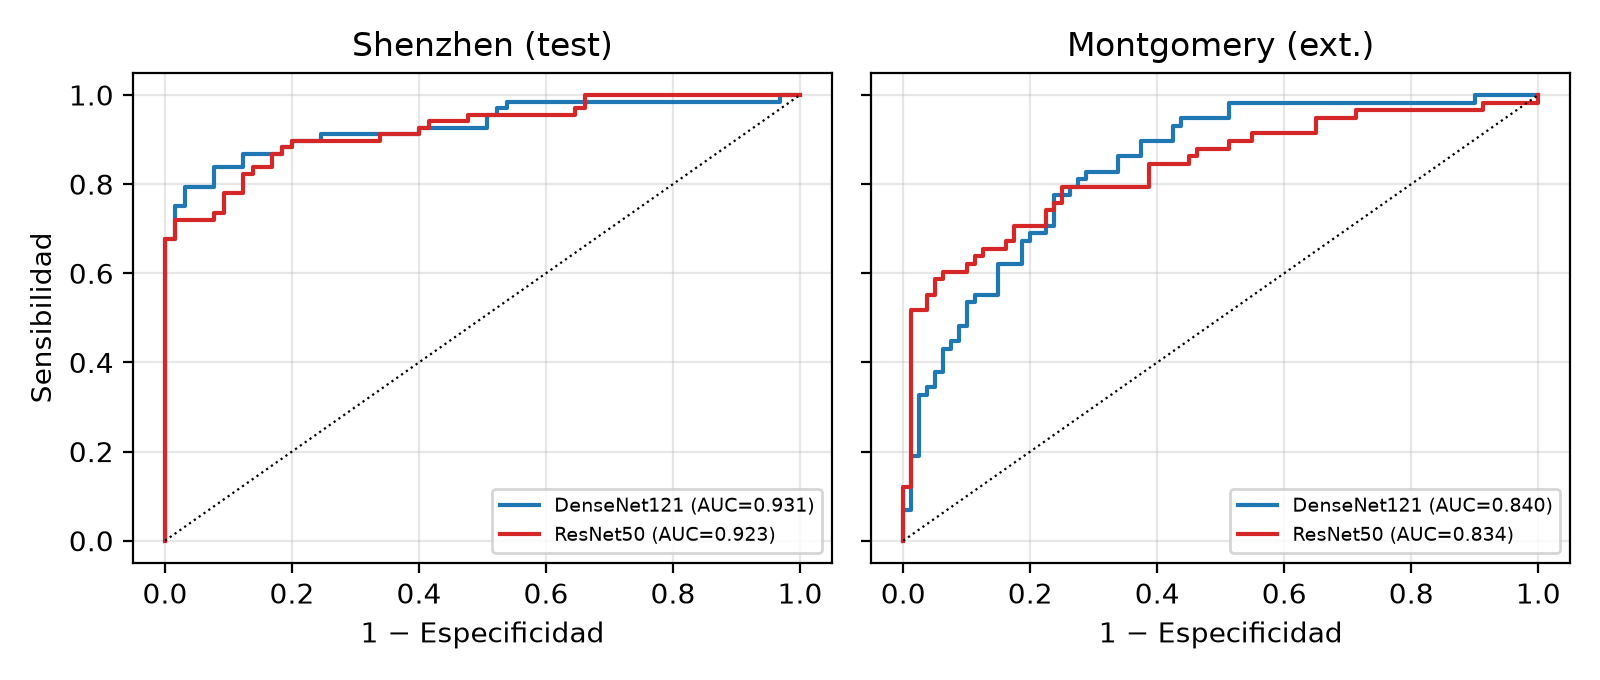
\includegraphics[width=.95\columnwidth]{fig_roc.png}
\caption{Curvas ROC históricas de la semilla 0 en Shenzhen y Montgomery. La elección del umbral se hizo solo en validación interna.}\label{fig:roc}\end{figure}

\begin{table}[t]\centering\caption{Clasificación histórica: media $\pm$ desviación entre tres semillas. Sensibilidad y especificidad usan el umbral de validación de cada modelo y semilla.}\label{tab:performance}\footnotesize
\begin{tabular}{llccc}\toprule
Modelo & Prueba & AUC & Sens. & Espec.\\\midrule
DenseNet121 & Shenzhen & .938$\pm$.007 & .77$\pm$.03 & .93$\pm$.02\\
DenseNet121 & Montgomery & .850$\pm$.039 & .61$\pm$.26 & .82$\pm$.19\\
ResNet50 & Shenzhen & .930$\pm$.006 & .75$\pm$.10 & .96$\pm$.04\\
ResNet50 & Montgomery & .792$\pm$.057 & .48$\pm$.18 & .87$\pm$.20\\\bottomrule
\end{tabular}\end{table}

\begin{table*}[t]\centering\caption{Métricas ampliadas de clasificación de la semilla 0, derivadas de las predicciones por radiografía. AP: precisión promedio; MCC: coeficiente de Matthews; Brier: error cuadrático medio de probabilidad. La matriz se ordena TN/FP/FN/TP. Los umbrales se fijaron en validación de Shenzhen.}\label{tab:perf_extended}\footnotesize
\begin{tabular}{llcccccc}
\toprule
Modelo & Prueba & AUC & AP & F1 & MCC & Brier & TN/FP/FN/TP\\
\midrule
DenseNet121 & Shenzhen & 0.931 & 0.950 & 0.850 & 0.722 & 0.102 & 60/5/14/54\\
DenseNet121 & Montgomery & 0.840 & 0.779 & 0.738 & 0.513 & 0.181 & 49/31/6/52\\
ResNet50 & Shenzhen & 0.923 & 0.941 & 0.831 & 0.728 & 0.109 & 64/1/19/49\\
ResNet50 & Montgomery & 0.834 & 0.824 & 0.487 & 0.442 & 0.165 & 79/1/39/19\\
\bottomrule
\end{tabular}\end{table*}

En los 55 positivos anotados de Montgomery, la ganancia media histórica de Grad-CAM dentro de cajas, condicionada al pulmón, fue 1,39 (IC 1,17--1,60) para DenseNet121 y 1,29 (1,13--1,44) para ResNet50, frente a aproximadamente 0,99 para mapas aleatorios suavizados. Se obtuvieron 157/165 y 165/165 mapas no nulos; la tasa de acierto del máximo fue 0,13 y 0,05. La aleatorización global de los pesos en la semilla 0 produjo correlaciones espaciales medianas de $-0,17$ y $-0,35$ respecto de los mapas entrenados, respectivamente. En el análisis general histórico de EIL, Grad-CAM y LIME de la clase predicha tuvieron Wilcoxon pareado $p=0,0014407984$ y $p=5,8444\times10^{-9}$ para DenseNet121 y ResNet50 (40 casos). La salida ejecutada redondeaba el segundo valor a cuatro decimales; ningún valor $p$ fue cero. La interpretación de esa comparación queda restringida por la clase objetivo distinta del análisis de cajas.

La Fig.~\ref{fig:historicxai} ilustra la dispersión de EIL del subconjunto histórico de 40 imágenes. La línea de referencia representa una fracción de área pulmonar aproximada de 0,26 para esa cohorte. Para un mapa uniforme, la referencia correcta es la fracción de cada radiografía; el promedio solamente facilita la lectura de la figura. Una EIL superior a esa referencia indica mayor concentración pulmonar que la esperada por área, pero no distingue señal patológica de estructuras normales dentro del pulmón. De manera análoga, la ganancia condicionada al pulmón puede superar uno aunque el máximo del mapa no caiga sobre la caja. La combinación observada de ganancia superior al control aleatorio y baja tasa de acierto del máximo muestra precisamente que las dos métricas responden a aspectos espaciales diferentes. También se debe considerar que un mapa de Grad-CAM suele provenir de una rejilla de activación mucho más gruesa que los 224$\times$224 píxeles de la entrada; la interpolación crea una apariencia suave que no recupera resolución perdida.

La Tabla~\ref{tab:perf_extended} permite examinar las métricas adicionales junto con las matrices de confusión de la semilla 0. En Montgomery, la AP de DenseNet121 fue 0,779 y su F1 fue 0,738, mientras que ResNet50 obtuvo AP 0,824 y F1 0,487 al umbral trasladado. El orden opuesto de AP y F1 en ese ejemplo refleja que AP resume posiciones de todos los umbrales y F1 depende del umbral fijo. Asimismo, el MCC de 0,513 frente a 0,442 incorpora verdaderos negativos además de aciertos positivos. La puntuación de Brier de 0,181 frente a 0,165 describe error probabilístico; no se infiere de esa diferencia una calibración global superior sin curvas de confiabilidad e intervalos adecuados.

\begin{figure}[t]\centering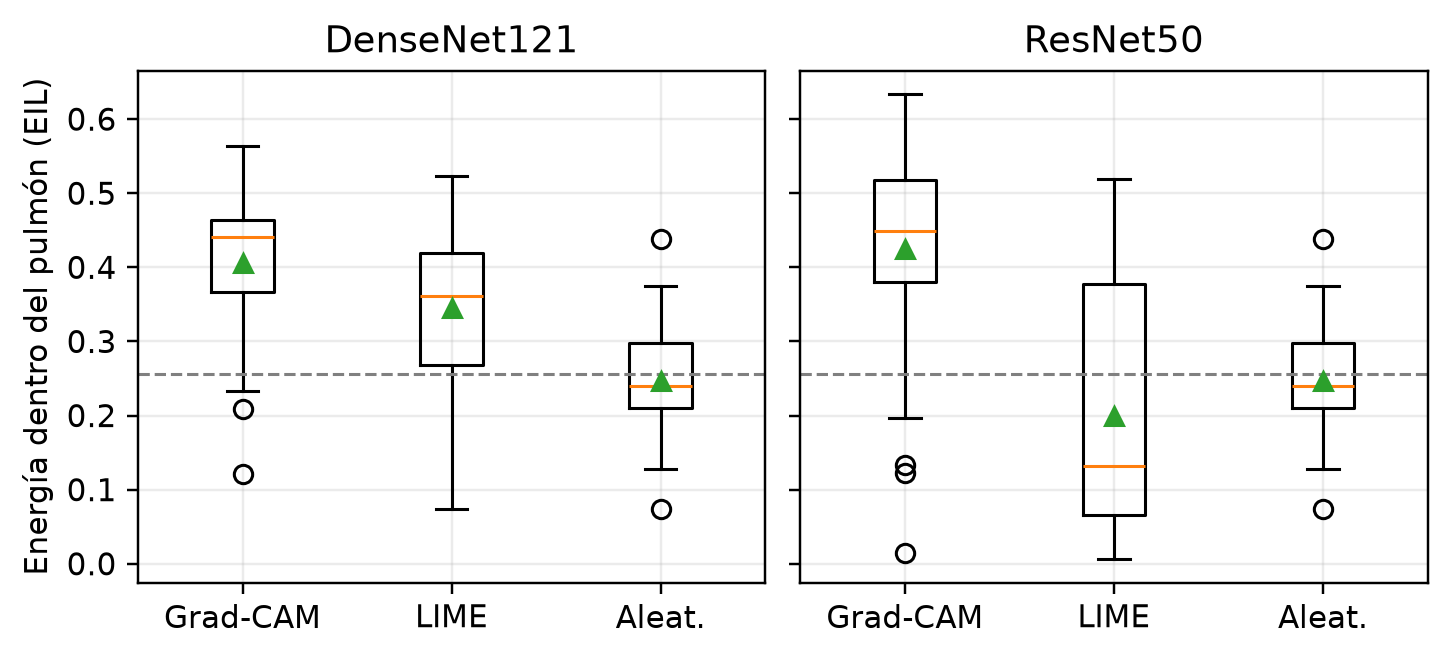
\includegraphics[width=.88\columnwidth]{fig_xai_box.png}
\caption{EIL histórica por método en 40 radiografías de Montgomery y semilla 0. La línea indica la fracción pulmonar media aproximada; la referencia uniforme es individual.}\label{fig:historicxai}\end{figure}

\subsection{Ejemplos de explicaciones de la clase positiva}
La Fig.~\ref{fig:lungdense} presenta dos casos elegibles de Montgomery con DenseNet121, semilla 0. MCUCXR\_0142\_1.png se clasificó como positivo y MCUCXR\_0182\_1.png fue un falso negativo al umbral fijado en Shenzhen. En ambos, Grad-CAM se calculó para la clase TB positiva, con independencia de la decisión. En el falso negativo, la zona más intensa queda lejos de la caja índice: un color intenso no confirma la localización de un hallazgo. Los mosaicos completos de cuatro casos, Grad-CAM y LIME para ambas arquitecturas se conservan en los resultados del proyecto. En ResNet50, esos cuatro casos recibieron una decisión negativa al umbral de la semilla 0. Las regiones coloreadas de LIME fuera del pulmón y la difusión de Grad-CAM muestran posibles áreas de atención, no diagnósticos ni una comparación cuantitativa entre métodos.

\begin{figure}[t]
\centering
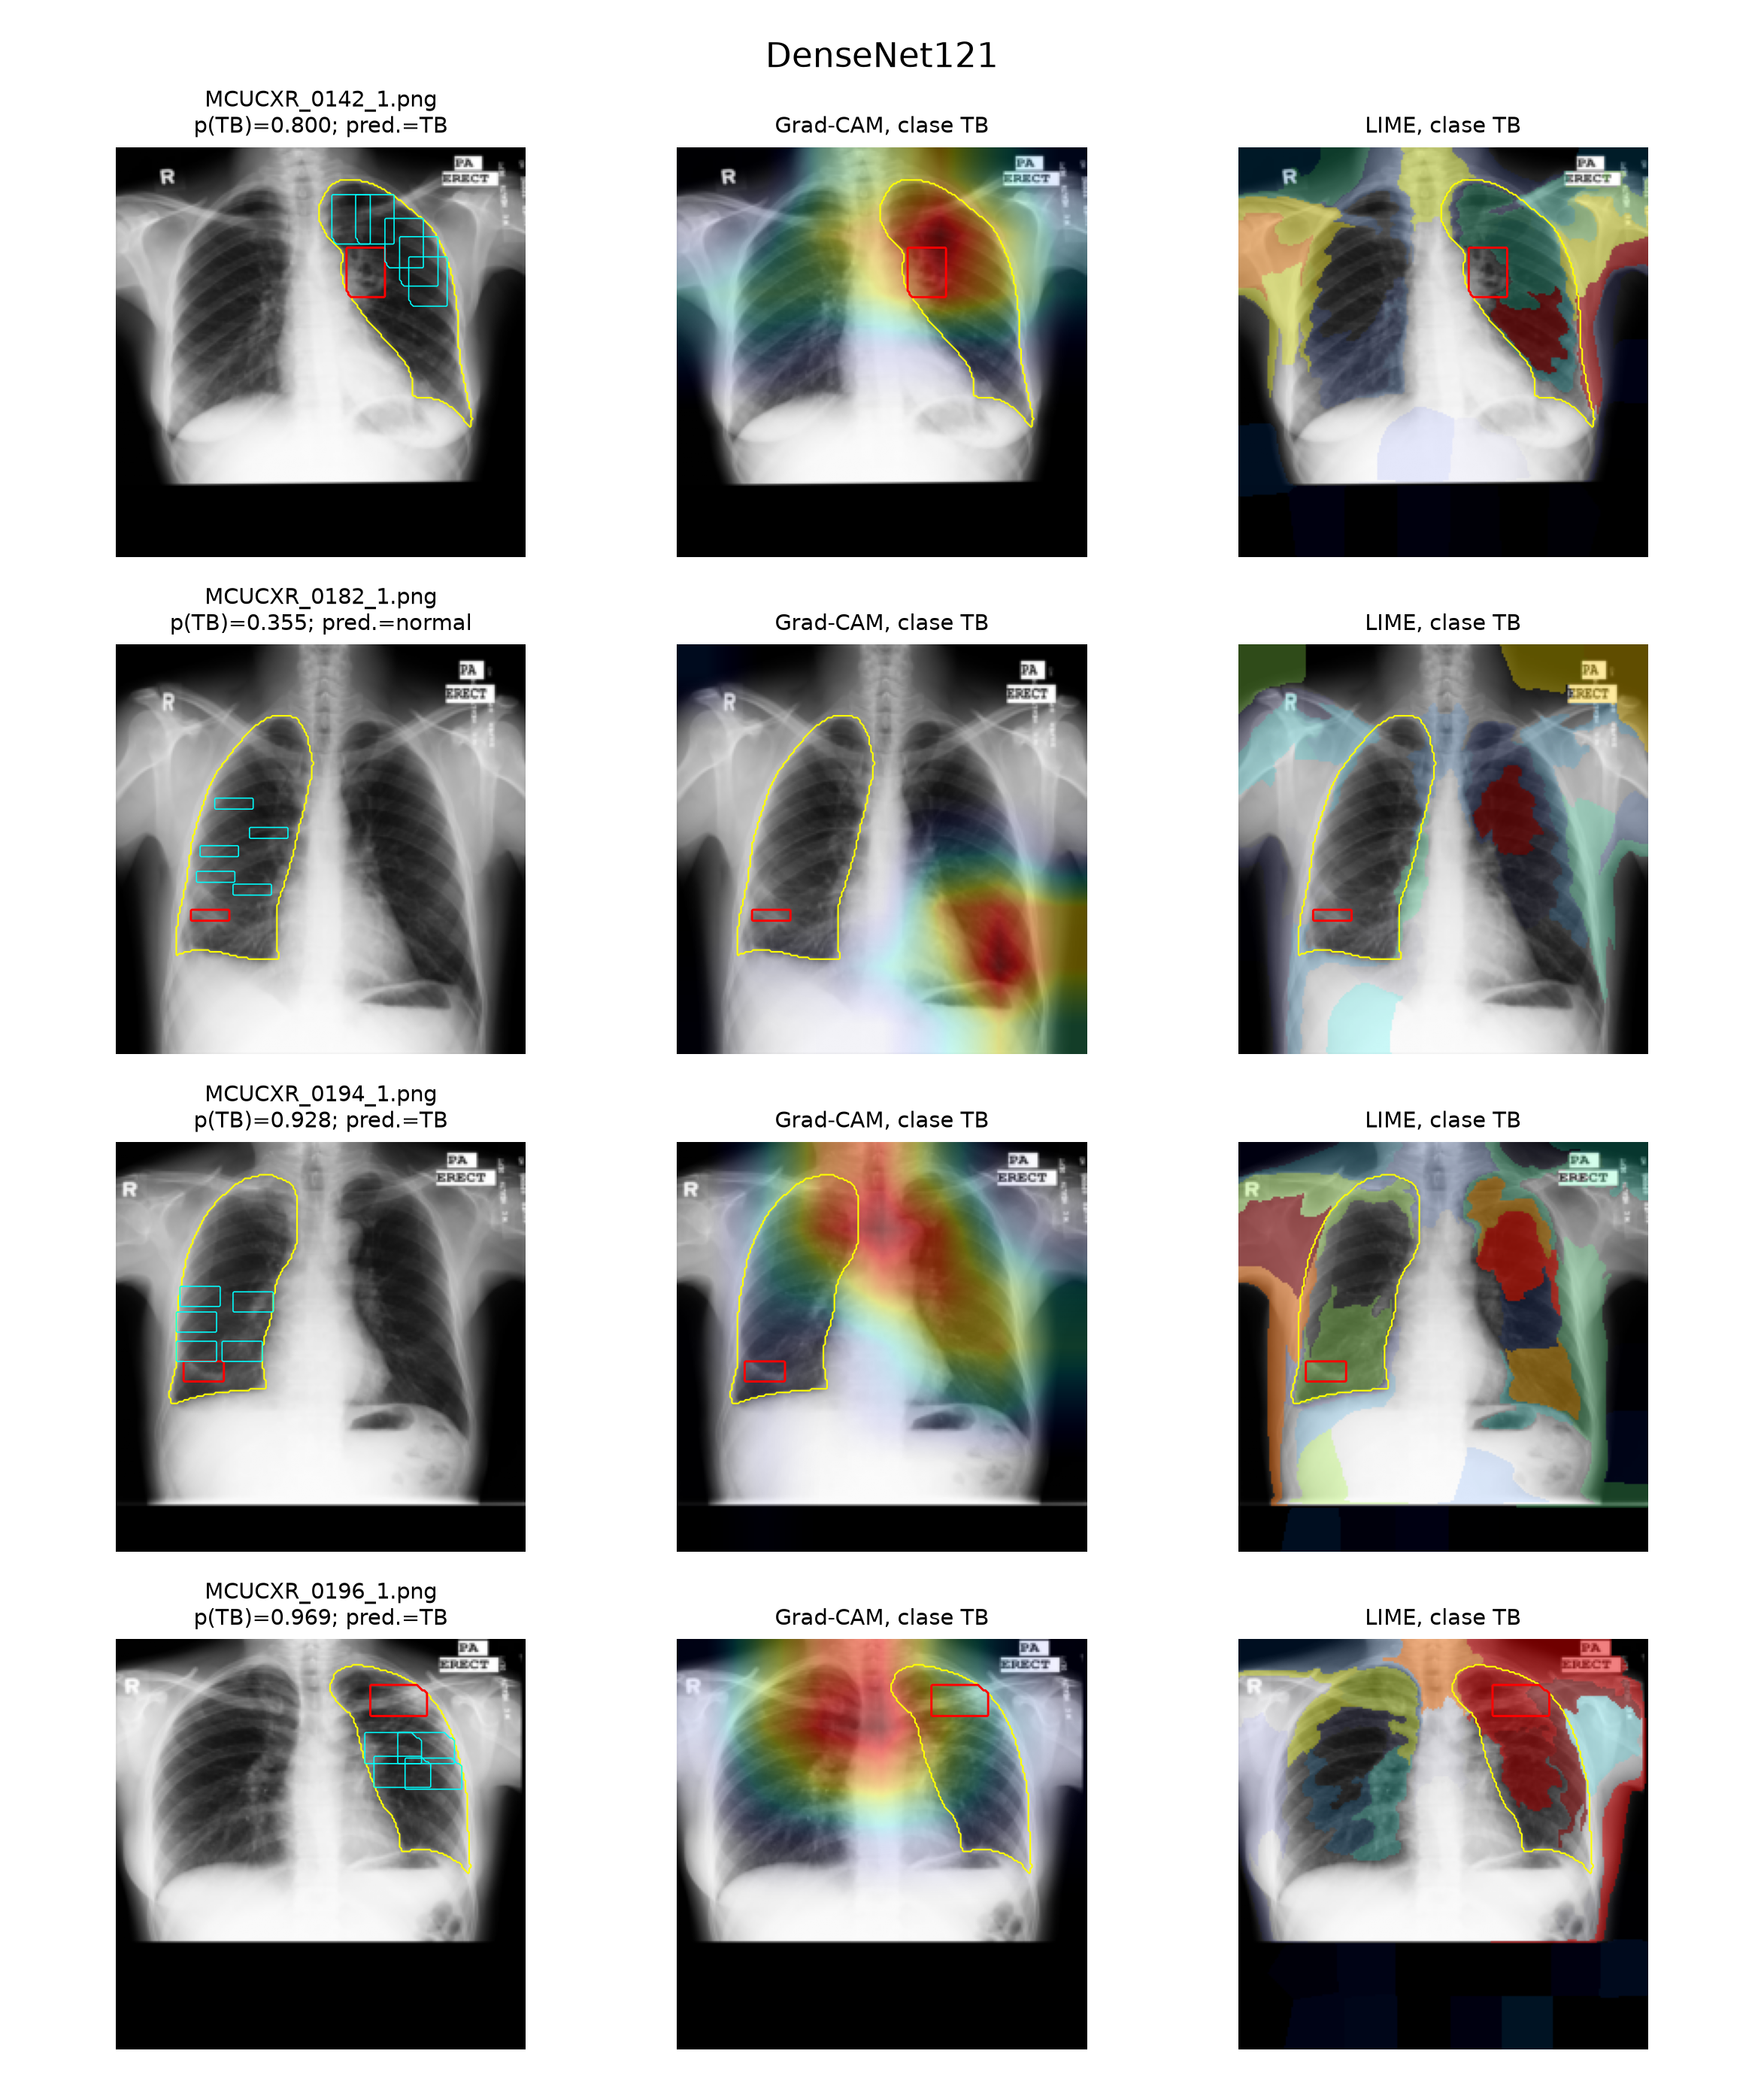
\includegraphics[width=.48\columnwidth,trim=48bp 632bp 516bp 61bp,clip]{fig_lung_xai_densenet121.png}\hfill
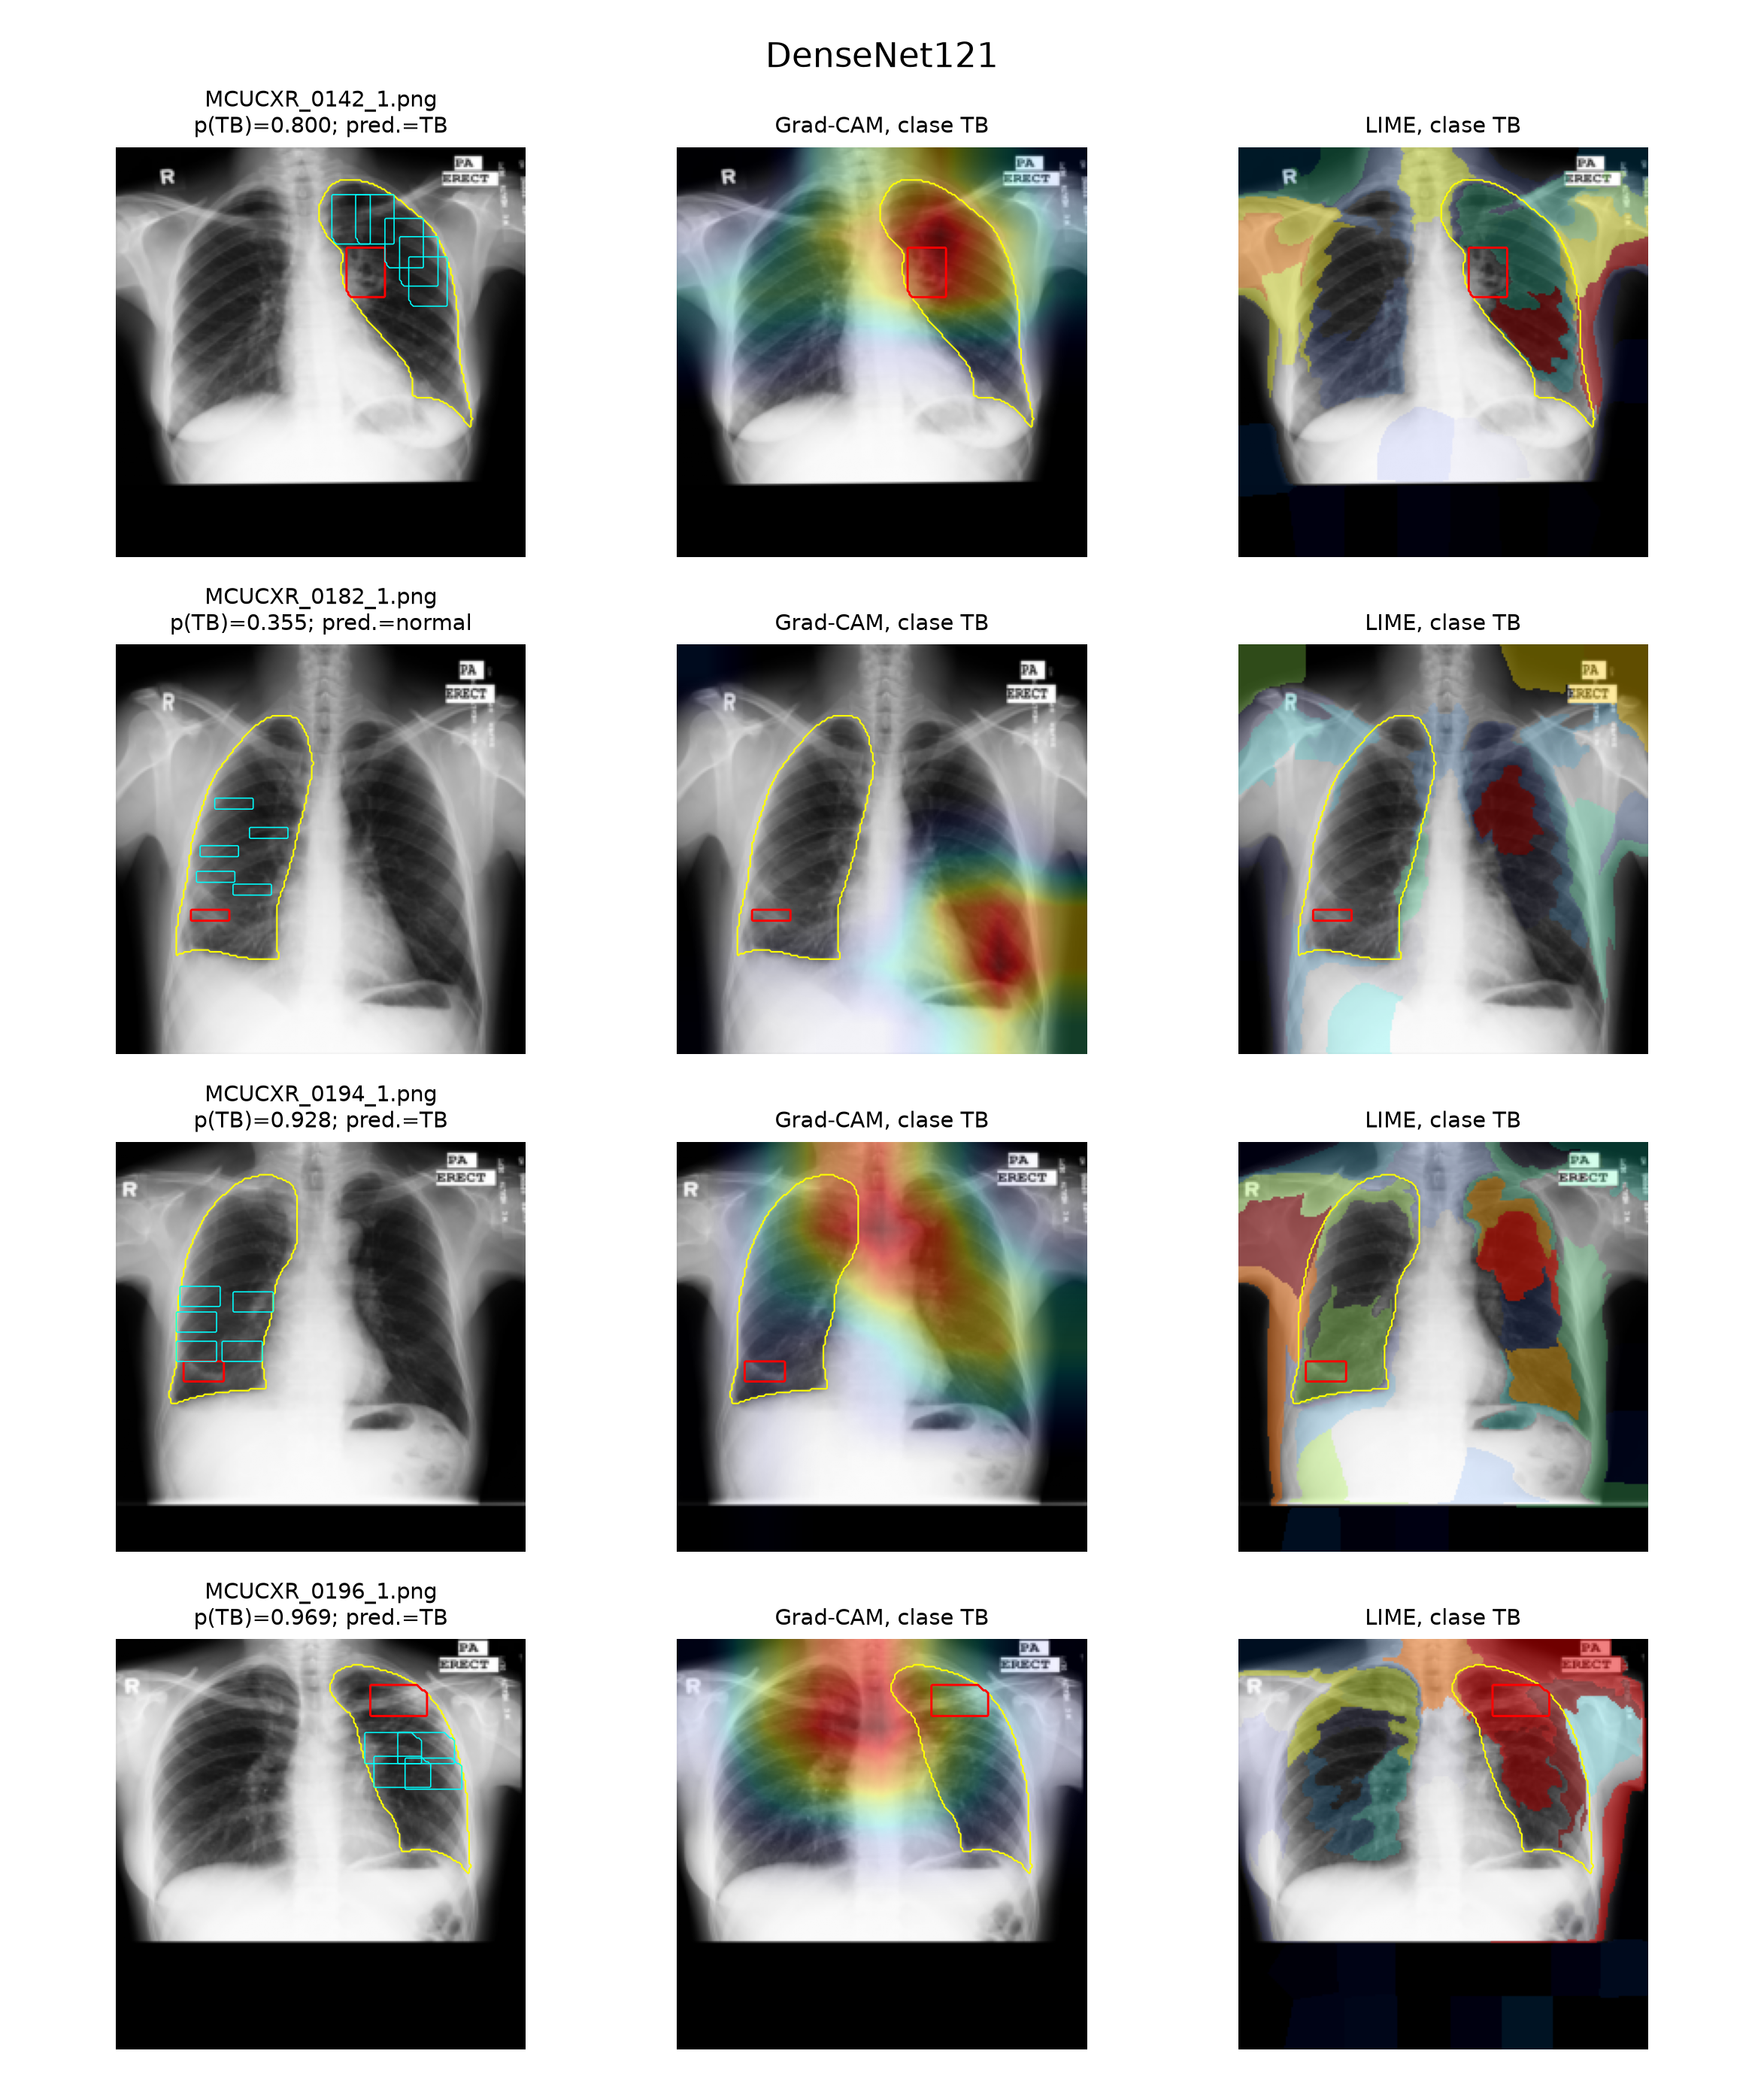
\includegraphics[width=.48\columnwidth,trim=282bp 632bp 282bp 61bp,clip]{fig_lung_xai_densenet121.png}\\[2pt]
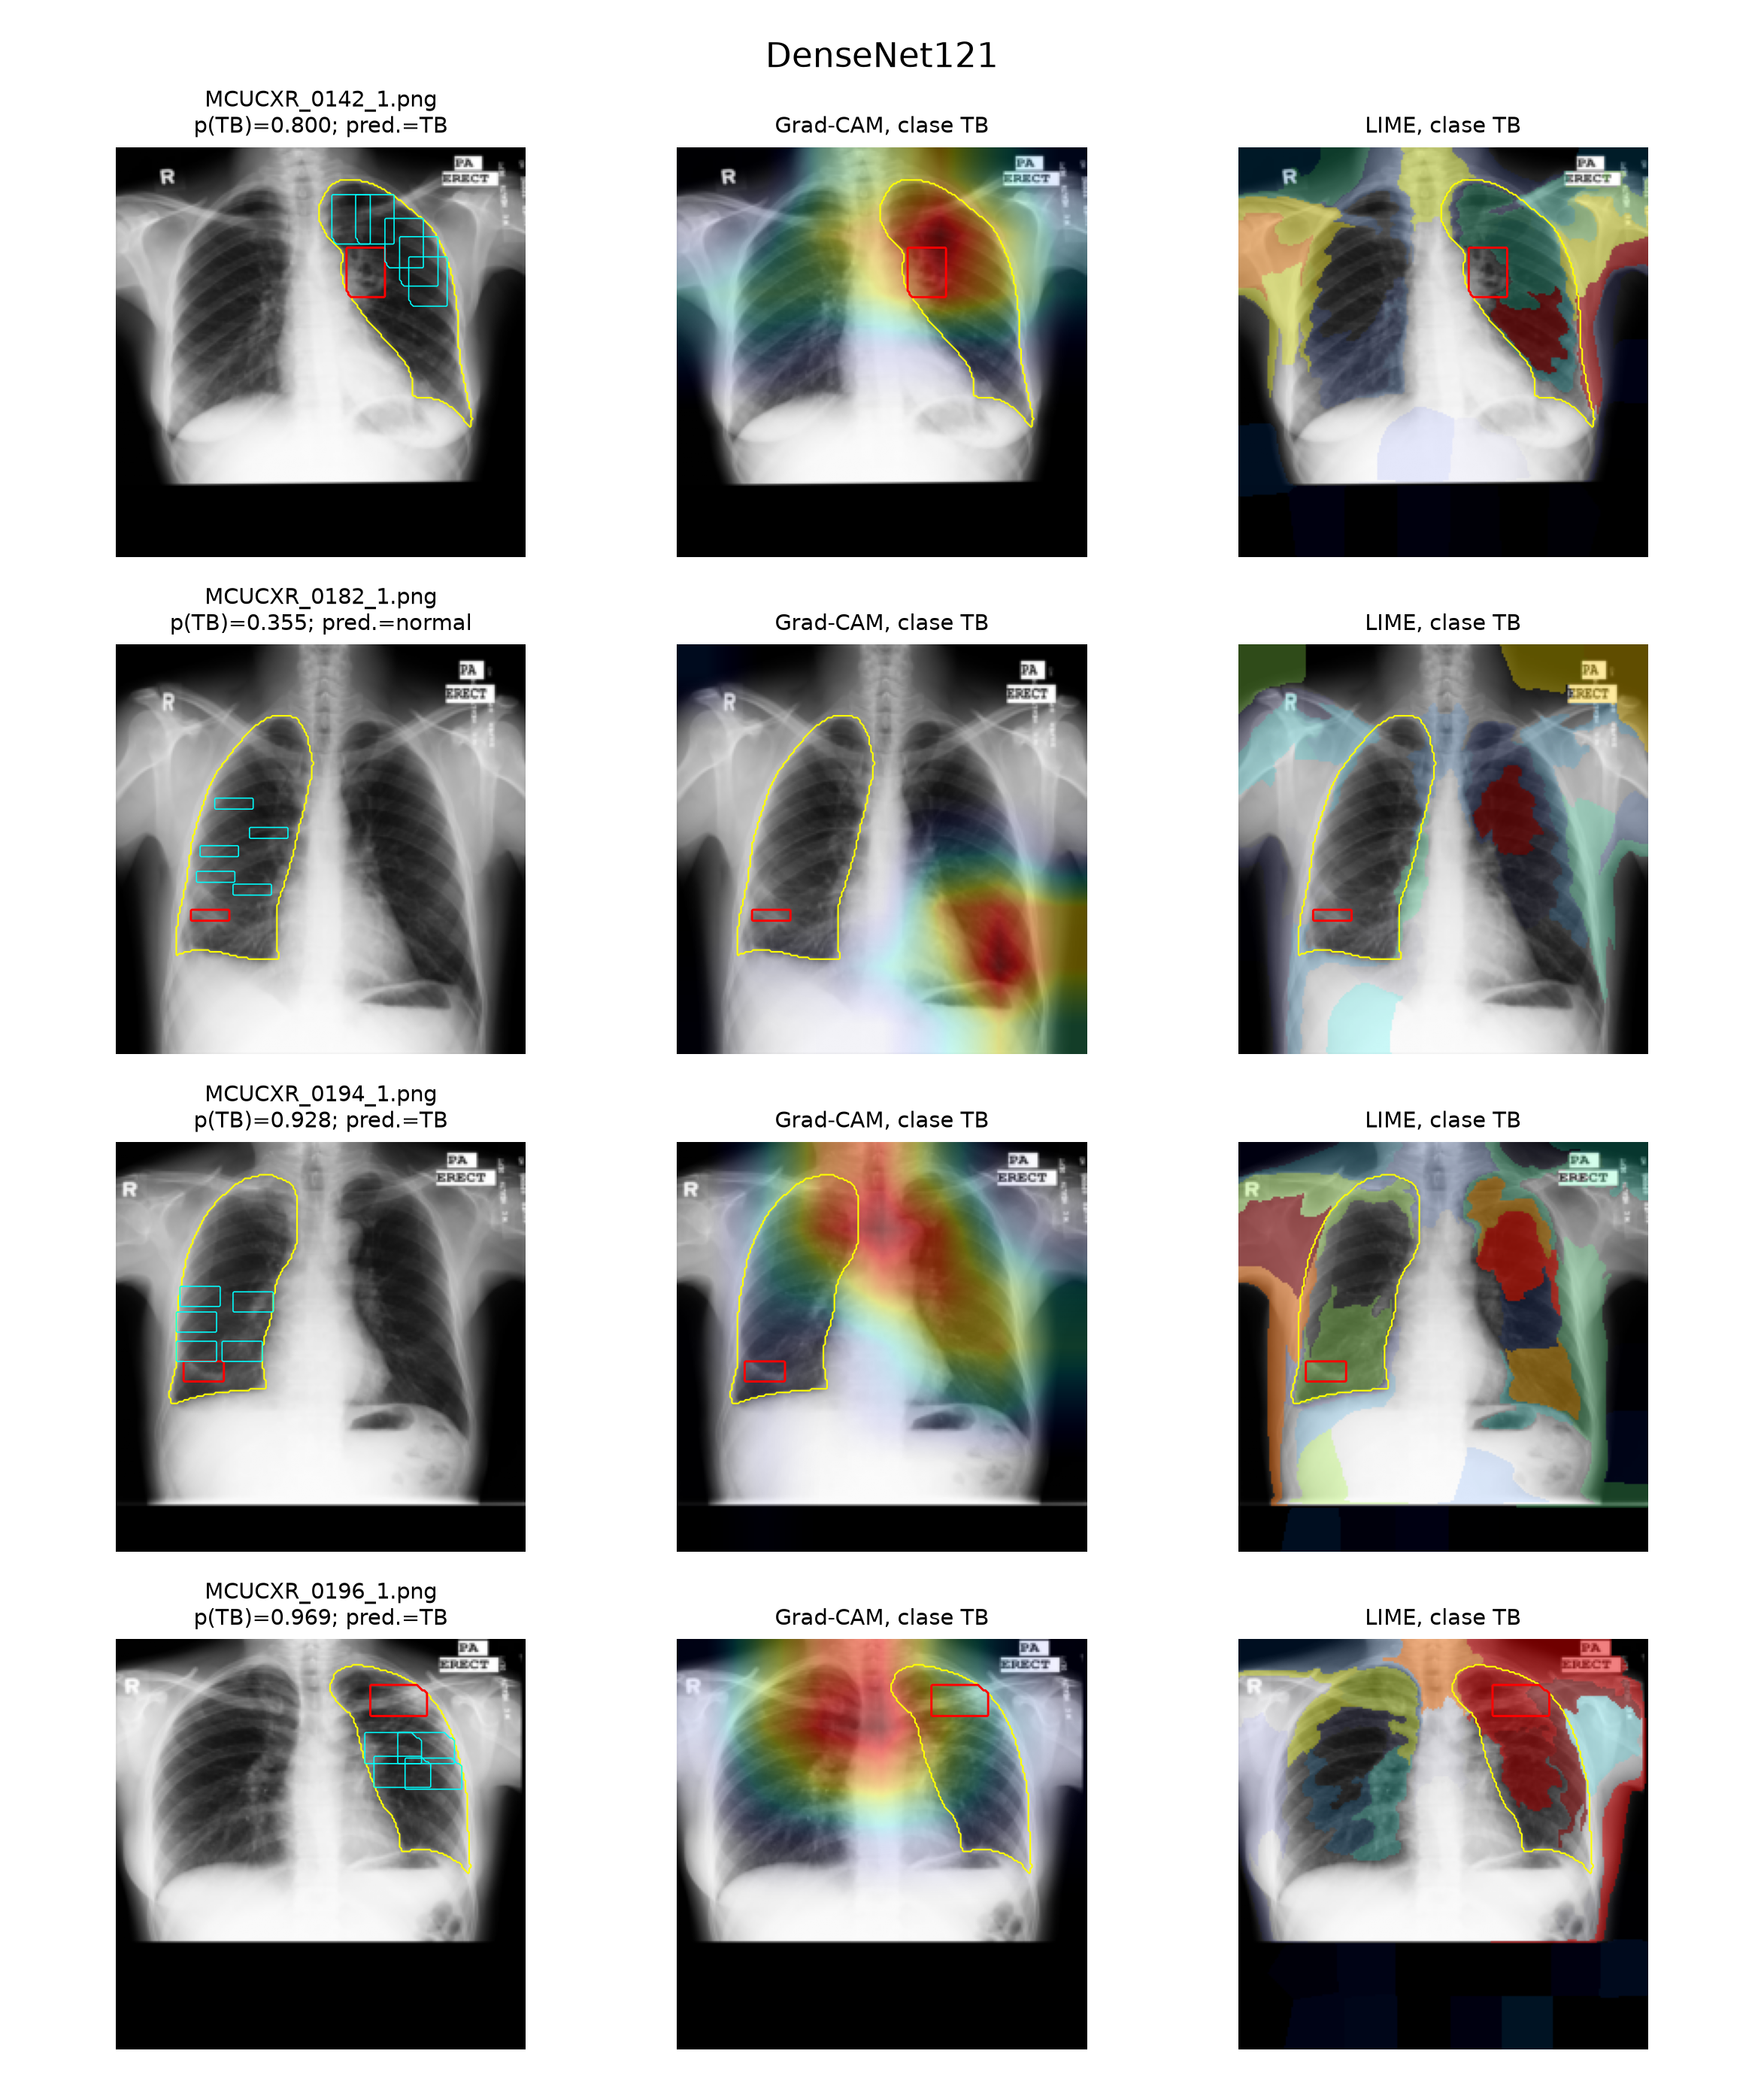
\includegraphics[width=.48\columnwidth,trim=48bp 425bp 516bp 268bp,clip]{fig_lung_xai_densenet121.png}\hfill
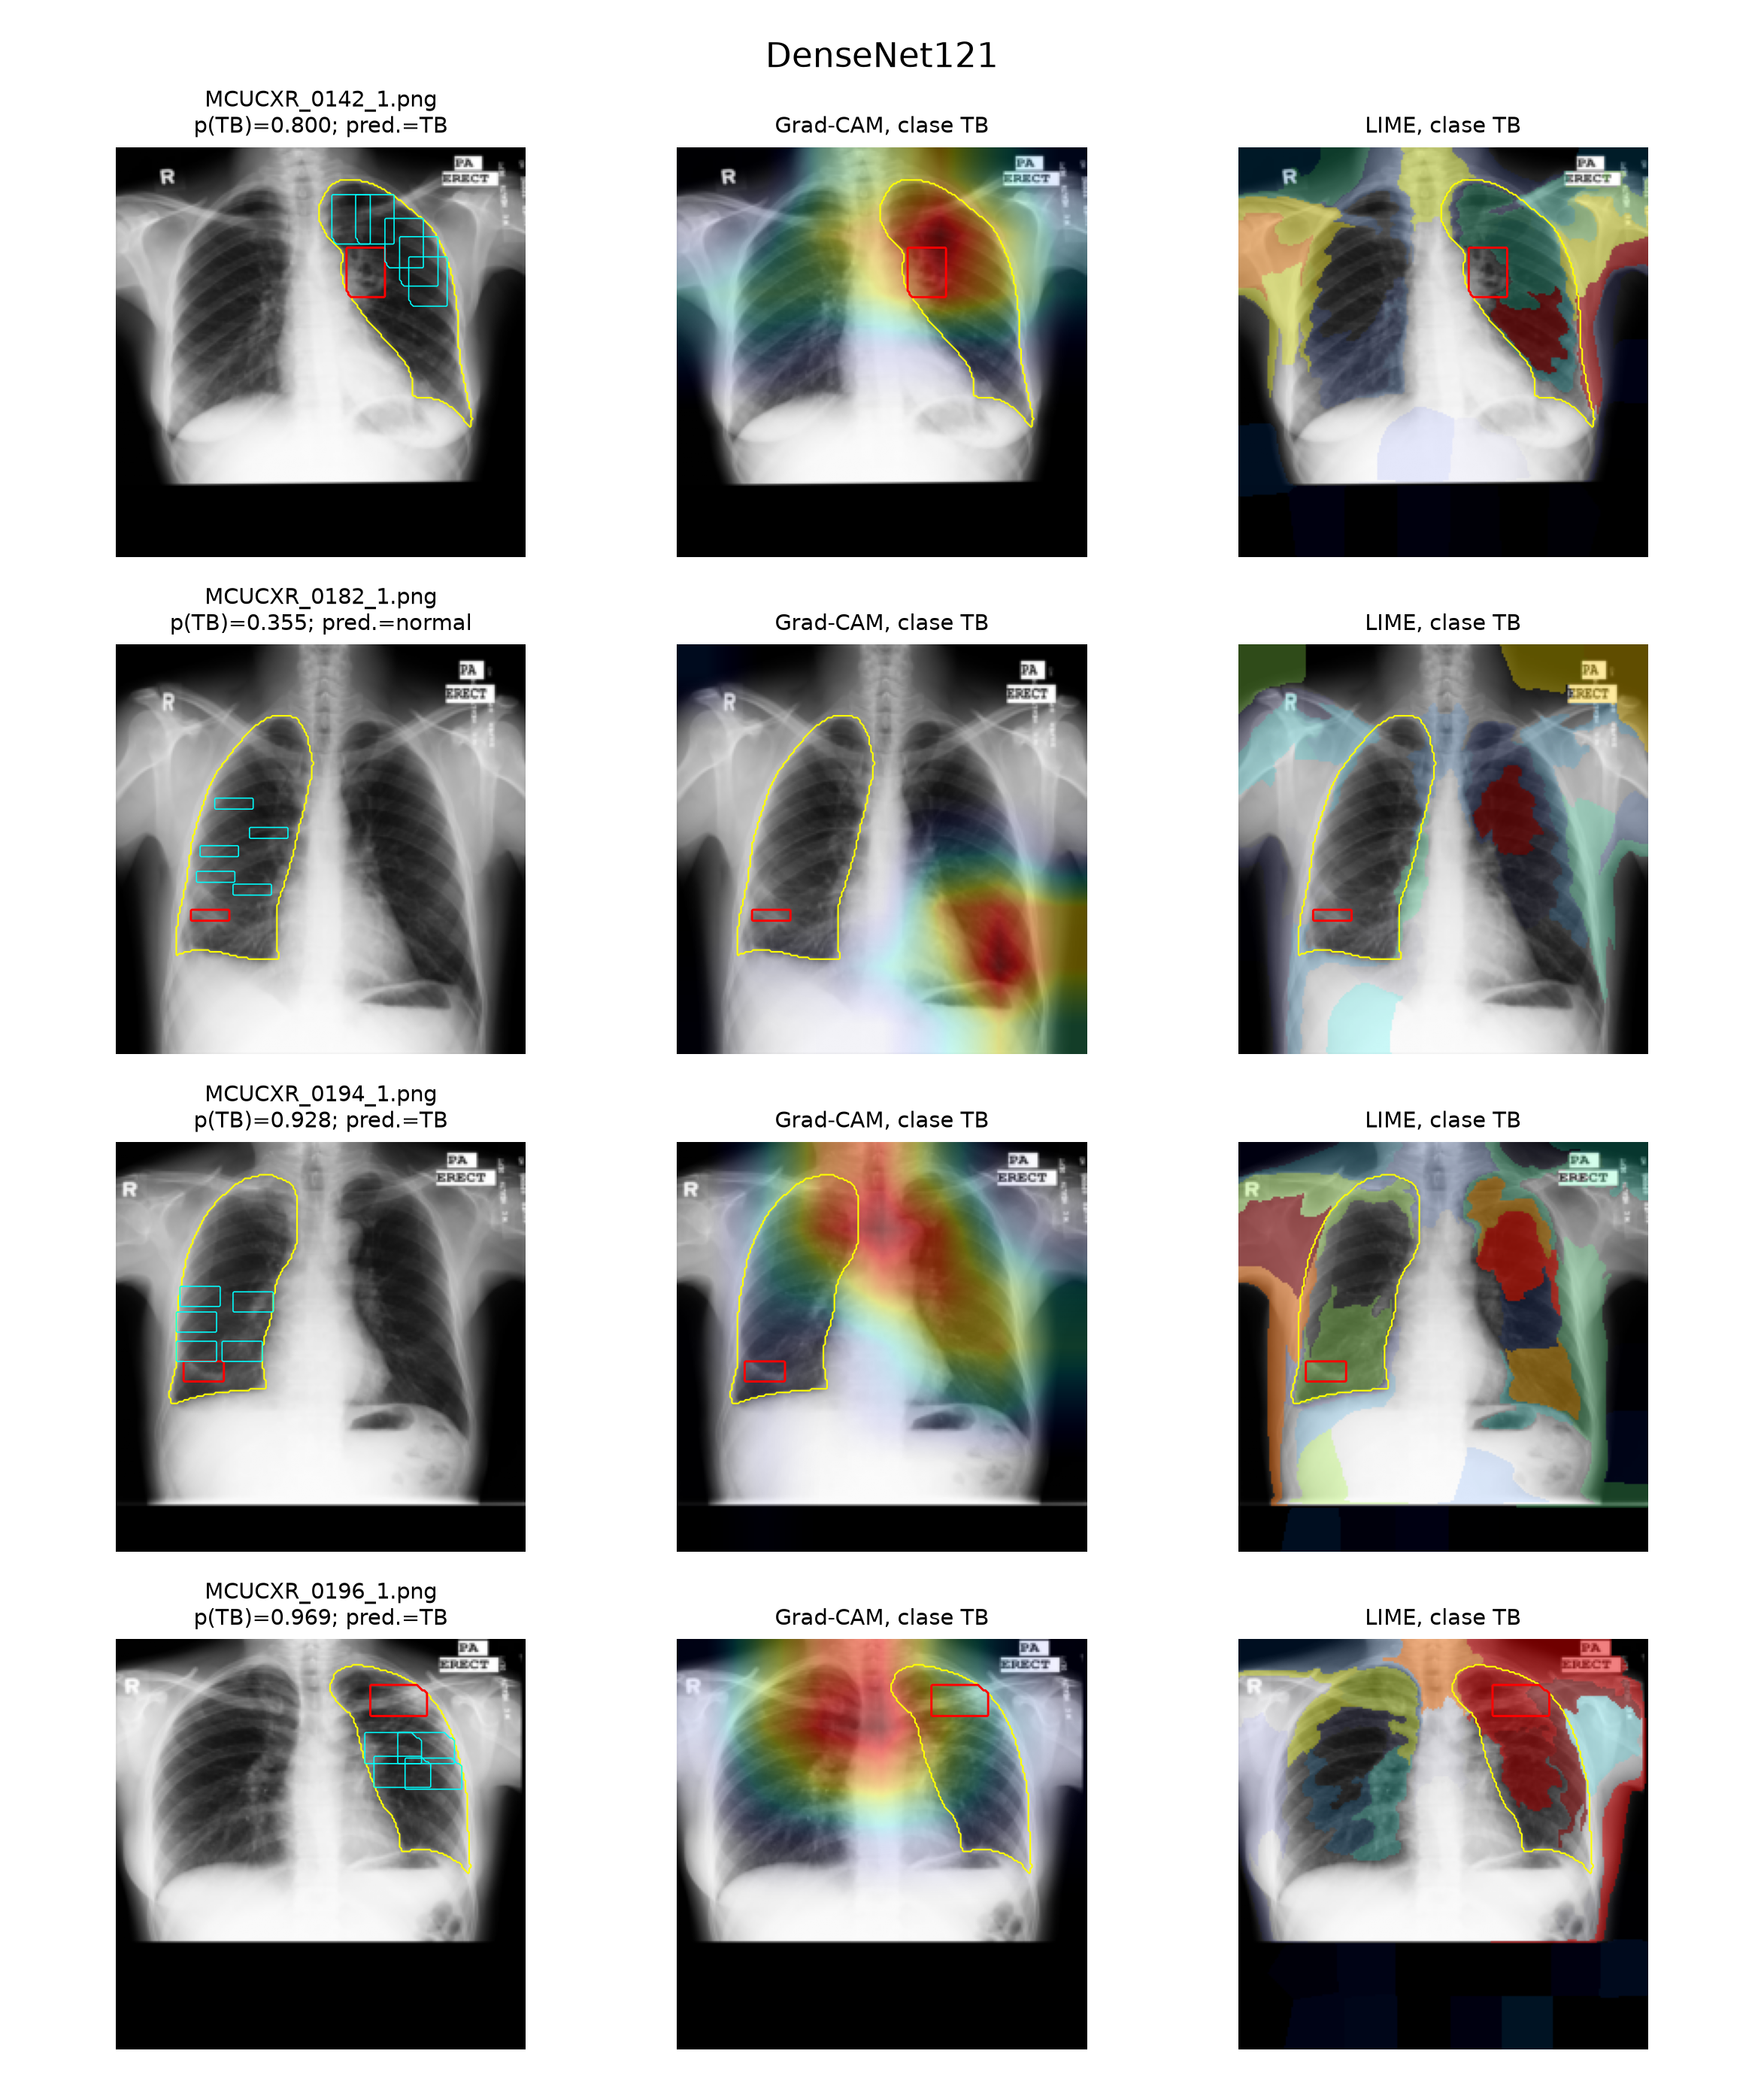
\includegraphics[width=.48\columnwidth,trim=282bp 425bp 282bp 268bp,clip]{fig_lung_xai_densenet121.png}
\caption{Dos radiografías de Montgomery con DenseNet121 (semilla 0). Arriba: caso positivo bien clasificado MCUCXR\_0142\_1; abajo: falso negativo MCUCXR\_0182\_1. Izquierda: radiografía con pulmón (amarillo), caja índice (rojo) y controles (cian). Derecha: Grad-CAM de la clase TB positiva para el mismo caso.}\label{fig:lungdense}
\end{figure}

\subsection{Contraste intrapulmonar nuevo}
La Tabla~\ref{tab:matched} y la Fig.~\ref{fig:matched} presentan el contraste nuevo. En DenseNet121, 13 de 17 radiografías tuvieron $D>0$. La mediana fue 0,172 (IC 0,065--0,632), estadístico de Wilcoxon 24 y $p=0,010986$. La prueba de signos fue $p=0,049042$ y la correlación biserial 0,686. En ResNet50, 12 de 17 tuvieron $D>0$; la mediana fue 0,064 (IC $-0,005$--0,336), con Wilcoxon $p=0,026672$ y prueba de signos $p=0,143463$. El intervalo de la mediana y la prueba de signos no apoyan una dirección estable en ese análisis de sensibilidad. El cambio mediano de probabilidad índice menos controles fue 0,0186 (IC 0,0042--0,0744) y 0,0113 (IC $-0,0008$--0,0668), respectivamente. Para $\sigma=5$, las medianas de $D$ fueron 0,192 y 0,106; se conservan en el archivo de resultados con sus valores $p$ crudos y ajustados.

\begin{table}[t]\centering\caption{Contraste de lesión frente a regiones sin anotación, $\sigma=10$. Se promedian tres semillas por radiografía; IC bootstrap del 95\%. Solo DenseNet121 es principal.}\label{tab:matched}\footnotesize
\begin{tabular}{lccccc}
\toprule
Modelo & $n$ & Mediana $D$ [IC] & $W$ & $p$ & $r_{rb}$\\
\midrule
DenseNet121 & 17 & 0.172 [0.065,0.632] & 24 & 0.01099 & 0.686\\
ResNet50 & 17 & 0.064 [-0.005,0.336] & 30 & 0.02667 & 0.608\\
\bottomrule
\end{tabular}\end{table}

\begin{figure}[t]\centering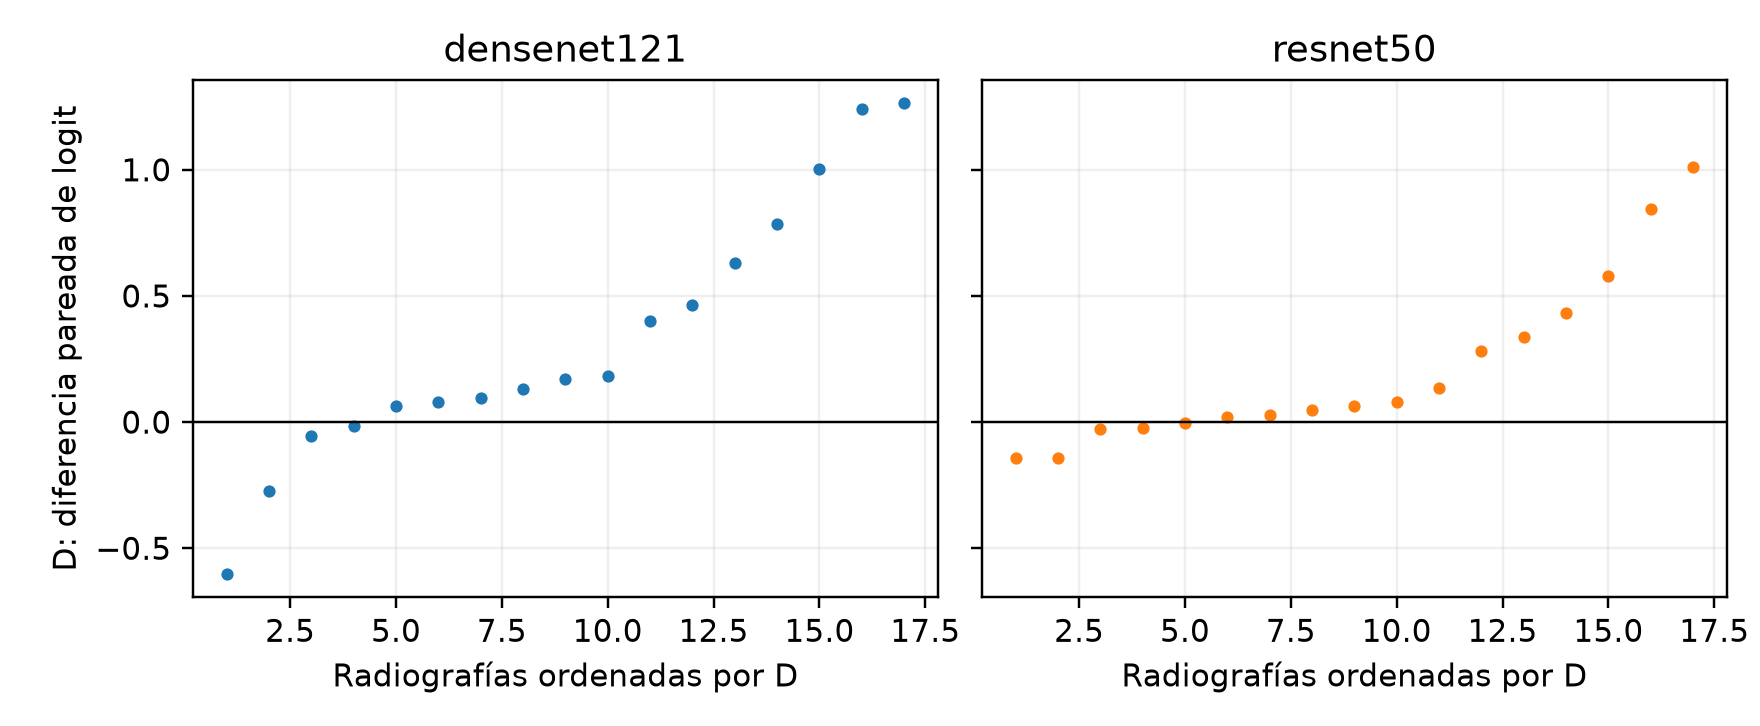
\includegraphics[width=.95\columnwidth]{fig_matched_d.png}
\caption{Valores $D$ por radiografía, ordenados dentro de cada arquitectura. La línea horizontal representa ausencia de diferencia.}\label{fig:matched}\end{figure}

La correlación de Spearman entre diferencia de masa Grad-CAM y $D$ fue 0,324 (IC bootstrap $-0,217$ a 0,773) en DenseNet121 y 0,287 ($-0,347$ a 0,764) en ResNet50. Estos intervalos amplios no establecen concordancia. La prueba de mapas mide asociación entre dos resúmenes calculados en las mismas imágenes, no fidelidad causal de cada píxel.

En los mapas válidos de la ampliación, el IoU medio del 10\% pulmonar superior con la región índice fue 0,038 para DenseNet121 y 0,045 para ResNet50, descriptivamente bajo. Se obtuvieron 42/51 y 51/51 mapas con masa pulmonar no nula, respectivamente, al considerar 17 radiografías y tres semillas a $\sigma=10$. Las áreas medias de eliminación e inserción fueron 0,387/0,344 para DenseNet121 y 0,558/0,551 para ResNet50. No se realizó inferencia entre arquitecturas con estas curvas. El mapa uniforme dio diferencia de masa índice menos controles exactamente cero, como corresponde a regiones de área igual dentro del pulmón; los mapas aleatorios suavizados promediaron 0,0012 y el mapa centrado $-0,0030$. El IoU de un mapa uniforme depende por completo del desempate de píxeles, por lo que no se interpretó como localización.

\subsection{Sensibilidad posterior a las reglas geométricas}
La elegibilidad baja motivó un análisis posterior que cambió únicamente dos tolerancias geométricas, sin utilizar las predicciones para escoger controles. Al admitir una diferencia media al borde de hasta 10 en vez de 5 píxeles y mantener la separación de centroides en 12, el número elegible aumentó de 17 a 23. Al reducir además esa separación a 6, aumentó a 26. Las nueve radiografías adicionales de la última versión incluyen las seis de la primera ampliación. La Tabla~\ref{tab:geometry} presenta resultados descriptivos de ambos modelos para las tres reglas. En DenseNet121 las medianas de $D$ fueron positivas en las tres; en ResNet50 también. Puesto que las reglas se flexibilizaron después del contraste inicial, los valores $p$ de estas versiones son exploratorios y no sustituyen el contraste principal prefijado.

\begin{table*}[t]\centering\caption{Sensibilidad geométrica posterior. Las reglas se expresan como tolerancia de distancia al borde/separación mínima de centroides en píxeles. IoU máx. med. es la mediana entre radiografías del máximo solapamiento de dos controles; la brecha es la mediana de la diferencia media de distancia al borde. Los $p$ de las dos reglas ampliadas son exploratorios y sin ajuste por selección de protocolo.}\label{tab:geometry}\footnotesize
\begin{tabular}{lccccccc}
\toprule
Reglas (borde/centros) & $n$ & DenseNet121: $D$ [IC] & $p$ & ResNet50: $D$ [IC] & $p$ & IoU máx. med. & Brecha borde med.\\
\midrule
5/12 & 17 & 0.172 [0.065,0.632] & 0.01099 & 0.064 [-0.005,0.336] & 0.02667 & 0.108 & 0.78 px\\
10/12 & 23 & 0.390 [0.132,0.632] & 0.00025 & 0.174 [0.026,0.476] & 0.00041 & 0.170 & 1.94 px\\
10/6 & 26 & 0.334 [0.079,0.495] & 0.00041 & 0.110 [0.029,0.442] & 0.00041 & 0.461 & 1.19 px\\
\bottomrule
\end{tabular}\end{table*}

La relajación aumentó también la similitud entre controles: el máximo IoU entre dos controles tuvo mediana 0,108 con las reglas principales, 0,170 con 10/12 y 0,461 con 10/6. La mediana de la brecha media respecto del borde fue 0,78, 1,94 y 1,19 píxeles, respectivamente. Los controles no se contaron como observaciones independientes en ninguna versión, pero su mayor solapamiento reduce la diversidad de regiones sin anotación. Una exploración geométrica más amplia mostró que 25 de las 54 imágenes con una caja índice válida no tenían ninguna traslación admisible dentro del mismo tercio vertical cuando se excluyeron las demás cajas, incluso sin restringir la distancia al borde. Once no tenían una traslación libre de cajas en ninguna altura del pulmón. Superar sustancialmente 26 casos exigiría modificar condiciones centrales del contraste, como el tercio vertical o la forma trasladada, y respondería a otra pregunta anatómica.

\subsection{Auditoría de resultados y controles históricos}
El manifiesto de particiones y el CSV de predicciones permitieron volver a calcular las matrices de confusión, ROC-AUC y los umbrales reportados. Los archivos de puntuaciones XAI conservaron identificadores, método y modelo, lo que permitió recuperar los valores de Wilcoxon de EIL sin depender de los textos redondeados del cuaderno ejecutado. Las exportaciones de la corrida rápida se mantuvieron en un directorio distinto y no se utilizaron en las tablas del presente artículo. Los pesos disponibles de las seis combinaciones de arquitectura y semilla se usaron únicamente para inferencia en la ampliación. El archivo de protocolo nuevo guarda reglas geométricas, semilla, resolución, intensidades de desenfoque, versión de SciPy, dispositivo y hash del CSV de cajas.

El análisis previo de perturbación comparó el marco exterior de cinco píxeles (8,73\% del área de imagen) con regiones de igual área dentro del pulmón en las 58 radiografías positivas de Montgomery. La caída media de probabilidad positiva al desenfocar una región pulmonar fue 0,262 (IC bootstrap 0,233--0,290) para DenseNet121 y 0,100 (0,078--0,124) para ResNet50; al desenfocar el borde las caídas fueron $-0,023$ y $-0,016$. Esos controles intrapulmonares eran campos aleatorios de área igual al borde y no estaban emparejados con cajas de hallazgos. La extensión actual responde a una pregunta más específica: si la alteración de una región marcada se distingue de la alteración de otras zonas de su mismo pulmón. Los valores numéricos de ambos experimentos no se compararon directamente porque difieren en área, selección de casos y unidad de control.

La revisión de correspondencia reveló una caja histórica mayoritariamente fuera de su máscara pulmonar. En el análisis antiguo se informó una sensibilidad excluyéndola; en la nueva selección se exigió antes de inferir que al menos la mitad de la caja índice quedara en un pulmón. La transformación de coordenadas de 1024 a 224 se aplicó de forma idéntica a todos los casos y el vecino más cercano evitó niveles intermedios en las máscaras. En la ampliación, el control de identidad usó una máscara vacía y verificó igualdad exacta de los píxeles de entrada. Para cada control se comprobó igualdad de área, inclusión en un solo pulmón y ausencia de solapamiento con la unión de cajas. Estas comprobaciones reducen errores de implementación, aunque no sustituyen una auditoría radiológica de cada región.

\subsection{Alcance estadístico de la ampliación}
El estadístico de rangos con signo supone simetría de la distribución de diferencias bajo la hipótesis nula; con 17 radiografías esa propiedad es difícil de evaluar con seguridad. Por ello se calculó la prueba exacta de signos, que solo utiliza la dirección, además de los rangos y de un IC bootstrap de la mediana. Para DenseNet121, ambas pruebas se situaron por debajo de 0,05, aunque la prueba de signos quedó cerca de ese límite. Para ResNet50, el valor $p$ de Wilcoxon fue 0,026672, pero su prueba de signos fue 0,143463 y el IC de la mediana incluyó cero. La evidencia secundaria, por tanto, fue menos estable frente al resumen estadístico empleado. El valor ajustado de Holm para ResNet50 a $\sigma=10$ fue 0,040314 dentro de la familia secundaria prefijada; este ajuste no elimina la discrepancia direccional ni la incertidumbre de selección.

Se evitó tratar las tres semillas como 51 observaciones o los hasta cinco controles como réplicas independientes. Cada radiografía aportó una sola diferencia, luego del resumen por controles y del promedio entre semillas. Los intervalos bootstrap remuestrearon las 17 radiografías completas y preservaron ese emparejamiento. El análisis no ajustó la elegibilidad respecto de características radiográficas no observadas; por ello los intervalos describen la variación de este subconjunto, no la de todas las radiografías con manifestaciones compatibles con TB. La correlación de Spearman también tuvo $n=17$ y se etiquetó exploratoria; los intervalos que cruzan cero impiden concluir que una mayor concentración del mapa prediga una mayor dependencia por perturbación.

\section{Discusión}
El contraste principal observó una caída mayor de la puntuación positiva al desenfocar la región anotada que al desenfocar regiones sin anotación de igual forma en el mismo pulmón. Este diseño controla área, anatomía lateral, tercio vertical y distancia aproximada al borde, y extiende el contraste histórico entre pulmón y borde. La diferencia de logit es una medida de dependencia de la red bajo el operador escogido; su magnitud no se traduce directamente en riesgo clínico. La prueba de signos fue limítrofe y el IC bootstrap se calculó con 17 unidades, por lo que conviene interpretar el valor $p$ junto con la dirección, el tamaño y la incertidumbre.

La mayor limitación es la selección geométrica: solo 17/55 positivos anotados permitieron los controles prefijados. Las lesiones grandes o cercanas a otras cajas quedaron subrepresentadas. Las regiones sin anotación no se certificaron sanas. Las cajas de consenso son rectangulares y aproximadas; pueden incluir parénquima normal o excluir hallazgos. Tampoco se inspeccionó sistemáticamente por especialistas cada región elegible. El redimensionado a 224$\times$224 y la resolución de Grad-CAM limitan la precisión espacial. El desenfoque crea imágenes modificadas que pueden estar fuera de la distribución de entrenamiento, incluso cuando se mantiene el presupuesto de píxeles. El cambio de salida puede depender de textura, contexto o artefactos residuales, no solo de patología.

La cohorte externa se había utilizado en el borrador histórico y no proporciona una validación independiente nueva de la hipótesis. Las tres semillas representan variación del entrenamiento, pero comparten imágenes y no son réplicas independientes. La ausencia de identificador independiente de paciente limita la auditoría de dependencia. Los conjuntos son pequeños y sus etiquetas son retrospectivas radiográficas, sin verificación microbiológica caso por caso en este análisis. Por ello el AUC, la localización y la sensibilidad a perturbaciones no constituyen evaluación clínica de un dispositivo. TBX11K contiene cajas de hallazgos en un diseño de detección distinto \cite{liu2020}; una extensión allí exigiría verificar equivalencia de etiquetas, licencias, duplicados, particiones y máscaras pulmonares validadas. Las máscaras anatómicas de conjuntos de COVID-19 no sustituirían anotaciones de lesión de TB.

\subsection{Procedencia, permisos y replicación}
La página oficial de NLM describe las colecciones como radiografías desidentificadas, con revisión ética para su uso y compartición en investigación, y especifica que las imágenes anormales contienen manifestaciones compatibles con TB \cite{nlmdata}. La copia de Kaggle se utilizó como canal de distribución de las radiografías; la atribución científica de datos y anotaciones corresponde a NLM y a sus publicaciones. La versión local observada fue la 1 del directorio de KaggleHub. Se conservaron hash de los CSV de consenso, un hash del manifiesto de rutas y tamaños y SHA-256 de cada una de las 800 radiografías. No se detectaron archivos de radiografía idénticos entre particiones; esto no excluye duplicados visuales transformados. La licencia específica de la copia Kaggle no pudo verificarse de forma concluyente a partir de los archivos locales examinados; antes de redistribuir imágenes o pesos derivados se requiere consultar las condiciones vigentes de ambas fuentes. El artículo y el cuaderno no incorporan credenciales de descarga.

La replicación exacta del análisis nuevo requiere mantener las particiones y checkpoints históricos, los CSV oficiales NLM, la geometría de 224$\times$224, las reglas de selección anteriores y los valores $\sigma=10$ y 5. El manifiesto de elegibilidad se produce antes de la inferencia y contiene los 55 identificadores anotados, motivo de exclusión, pulmón, área índice, número de controles y diferencias de distancia al borde. El CSV de puntuaciones registra cada radiografía, arquitectura, semilla e intensidad, junto con el cambio de logit, cambio de probabilidad y masa Grad-CAM. Otro CSV promedia por radiografía y el JSON conserva estadísticos completos. Esta secuencia permite recalcular el contraste sin contar semillas o controles como observaciones adicionales.

El cuaderno para Colab descarga imágenes mediante KaggleHub cuando no hay copia local, recupera los CSV desde las rutas oficiales de NLM, comprueba conteos y exporta predicciones, figuras y tablas. El modo rápido verifica la estructura técnica con menos épocas y menor resolución; queda separado del resultado empírico. La corrida de esta ampliación reutilizó los pesos de la corrida completa local. Por esa razón, el resultado nuevo verifica inferencia y análisis con esos archivos, mientras que el reentrenamiento íntegro en una sesión limpia de Colab permanece como una comprobación de replicación independiente. La variación entre bibliotecas, hardware o pesos de ImageNet puede producir cambios numéricos aun cuando el protocolo nominal sea el mismo.

\subsection{Diseño de una replicación posterior}
Para comprobar si el contraste observado se conserva fuera de Montgomery, una replicación deberá fijar primero la definición de caso positivo y comprobar su equivalencia con las etiquetas retrospectivas aquí usadas. Una colección con confirmación microbiológica permitiría examinar una pregunta clínica distinta, pero no sería una repetición directa sin armonizar definición de caso y distribución de pacientes. Deben obtenerse máscaras pulmonares independientes y anotaciones de hallazgos con convención de coordenadas explícita. La revisión radiológica de las regiones sin anotación ayudaría a estimar cuántos controles contienen señales no marcadas; una segunda lectura de las cajas índice permitiría cuantificar desacuerdo entre observadores. Una unidad de paciente estable resulta necesaria cuando existan exploraciones repetidas.

El protocolo debe registrarse antes de evaluar las salidas: arquitectura y pesos, intensidad de desenfoque, criterios de selección geométrica, mínimo de controles, contraste principal y familias secundarias. El conjunto de desarrollo debe definir transformaciones, parada temprana y umbrales, dejando la cohorte de replicación intacta hasta el análisis final. Se recomienda informar tanto la proporción elegible como las características de los excluidos, ya que una estimación favorable en lesiones pequeñas puede no generalizar a lesiones extensas. Deben conservarse resultados nulos, mapas inválidos y fallos de adquisición, y publicarse los valores $p$ completos junto con intervalos y tamaños de efecto. Una sensibilidad útil sería repetir el mismo presupuesto de píxeles con distintos fondos de sustitución, porque el desenfoque podría modificar texturas de manera diferente al relleno local o a la inpainting. Esa comparación mediría robustez al operador; aun si concordara, no convertiría una intervención digital en evidencia causal clínica.

Para evaluar utilidad de un sistema de cribado se necesitaría un diseño separado con referencia microbiológica, estimación de sensibilidad y especificidad en la población de uso, ajuste de umbral apropiado y evaluación prospectiva de flujo clínico. El estudio actual se limita a auditar una hipótesis sobre dependencia de clasificadores retrospectivos. Esta separación preserva el significado de las medidas XAI: localización, cambio de salida por perturbación y desempeño diagnóstico responden a preguntas diferentes y deben comunicarse con sus respectivas referencias y unidades de análisis.

\section{Conclusiones}
En una extensión retrospectiva de 17 radiografías geométricamente elegibles de Montgomery, DenseNet121 mostró una diferencia positiva de puntuación tras desenfocar hallazgos anotados frente a regiones sin anotación del mismo pulmón. El resultado fue más incierto para ResNet50 y la asociación con concentración de Grad-CAM no se estableció. La evidencia respalda el uso de contrastes pareados anatómicos para auditar hipótesis sobre dependencia del modelo; requiere replicación en una cohorte independiente, con anotaciones más completas y controles clínicamente revisados, antes de atribuirle significado diagnóstico.

\bibliographystyle{IEEEtran}
\bibliography{referencias}
\end{document}
